% ============================================================
%  CGAR — Multi-Agent Python Dependency Resolution | ML Course Project
% ============================================================
\documentclass[aspectratio=169,10pt]{beamer}

\usetheme{metropolis}
\usecolortheme{metropolis}
\usefonttheme{professionalfonts}
\setbeamertemplate{frame numbering}[fraction]
\setbeamertemplate{itemize item}{\textcolor{mLightBrown}{\tiny$\blacktriangleright$}}
% Clean presentation captions: no "Figure N:" label, grey italic
\setbeamertemplate{caption}{\centering\footnotesize\itshape\color{gray}\insertcaption\par}
\setbeamerfont{caption}{size=\footnotesize}

% -- Packages --
\usepackage{amsmath, amssymb}
\usepackage[utf8]{inputenc}
\usepackage{vietnam}
\usepackage[english]{babel}
\usepackage{booktabs}
\usepackage{multirow}
\usepackage[table]{xcolor}
\usepackage{graphicx}
\graphicspath{{figures/}}
\usepackage{hyperref}
\usepackage{listings}
\usepackage{parskip}
\usepackage{tikz}
\usetikzlibrary{arrows.meta, positioning, fit, backgrounds, decorations.pathreplacing, shapes.geometric, calc}
\usepackage{mdframed}
\usepackage{pifont}
\newcommand{\cmark}{\ding{51}}
\newcommand{\xmark}{\ding{55}}

% --- Semantic colored boxes (vay từ LeJEPA style) ---
\definecolor{cHard}{HTML}{B85450}      % terracotta: deterministic error
\definecolor{cSoft}{HTML}{C8A951}      % gold: probabilistic
\definecolor{cInfer}{HTML}{2C3E6B}     % navy: inferred / monotone
\definecolor{cUpper}{HTML}{2E86AB}     % steel blue: upper-bound constraint
\definecolor{cHardL}{HTML}{F2E6E5}
\definecolor{cSoftL}{HTML}{F5F0E0}
\definecolor{cInferL}{HTML}{EEF0F5}

\newmdenv[topline=false,bottomline=false,rightline=false,
  linewidth=2.5pt,linecolor=cHard,
  innerleftmargin=6pt,innerrightmargin=4pt,
  innertopmargin=3pt,innerbottommargin=3pt,
  backgroundcolor=cHardL]{hardbox}
\newmdenv[topline=false,bottomline=false,rightline=false,
  linewidth=2.5pt,linecolor=cSoft,
  innerleftmargin=6pt,innerrightmargin=4pt,
  innertopmargin=3pt,innerbottommargin=3pt,
  backgroundcolor=cSoftL]{softbox}
\newmdenv[topline=false,bottomline=false,rightline=false,
  linewidth=2.5pt,linecolor=cInfer,
  innerleftmargin=6pt,innerrightmargin=4pt,
  innertopmargin=3pt,innerbottommargin=3pt,
  backgroundcolor=cInferL]{inferbox}

% (removed unused \takeaway box macro — closing lines unified to one
%  centered \footnotesize\color{mDarkTeal} sentence style across the deck)

% Colors
\definecolor{mDarkTeal}{HTML}{23373B}
\definecolor{mLightBrown}{HTML}{EB811B}
\definecolor{softgray}{HTML}{F2F4F7}
\definecolor{tealtint}{HTML}{D6DEE0}
\definecolor{nightsky}{HTML}{18242B}   % gloomy night backdrop (darker mDarkTeal)
\definecolor{moongold}{HTML}{F3D55B}   % yellow moon

\colorlet{navydeep}{mDarkTeal}
\colorlet{accent}{mLightBrown}
\colorlet{success}{green!50!black}
\colorlet{alert}{red!70!black}

% Listings
\lstset{
  basicstyle=\ttfamily\scriptsize,
  keywordstyle=\color{mDarkTeal}\bfseries,
  commentstyle=\color{gray}\itshape,
  stringstyle=\color{mLightBrown!80!black},
  showstringspaces=false,
  frame=single,
  rulecolor=\color{tealtint},
  backgroundcolor=\color{softgray},
  breaklines=true,
  numbers=none,
  language=Python,
  xleftmargin=5pt,
  xrightmargin=5pt,
  aboveskip=7pt,
  belowskip=7pt,
}

% Title
\title{MEMRES to CGAR: Agentic Python Dependency Resolution}
\author{Trần Chí Nguyên, Đào Sỹ Duy Minh, Huỳnh Trung Kiệt}
\institute{University of Science, VNU-HCM}
\date{ML Course Project -- 2026}

\begin{document}

% ==================== TITLE ====================
\begin{frame}
\vspace{0.4em}
\begin{columns}[c]
\column{0.18\textwidth}
\centering
\href{https://www.hcmus.edu.vn}{
\includegraphics[height=2.0cm]{hcmus.png}}

\column{0.64\textwidth}
\centering
\LARGE\textbf{Machine Learning Course Project}\\[0.7em]
\large\textcolor{navydeep}{MEMRES $\to$ CGAR:\\Agentic Python Dependency Resolution}

\column{0.18\textwidth}
\centering
\href{https://conf.researchr.org/home/fse-2026}{
\includegraphics[height=1.6cm]{fse.png}}
\end{columns}

\vspace{1.5em}
\begin{columns}[c]
\column{0.45\textwidth}
\begin{block}{Project Overview}
\scriptsize
Khôi phục tự động môi trường Python từ mã nguồn cũ bằng \textbf{Multi-Agent LLM} và \textbf{Constraint Acquisition} (ràng buộc học dần từ build-verifier).
\end{block}

\column{0.4\textwidth}
\begin{block}{Team Members}
\scriptsize
\begin{itemize}
  \item Trần Chí Nguyên -- 23102244
  \item Đào Sỹ Duy Minh -- 23122041
  \item Huỳnh Trung Kiệt -- 23122039
\end{itemize}
\end{block}
\end{columns}

\vspace{1.1em}
\centering
\scriptsize University of Science, VNU-HCM
\end{frame}

% ==================== OUTLINE ====================
\begin{frame}{Nội dung chính}
\begin{enumerate}
  \item Bối cảnh \& Phát biểu bài toán
  \item Công trình liên quan \& Khoảng trống nghiên cứu
  \item MEMRES: Phương pháp nền tảng
  \item \textbf{\color{mLightBrown}CGAR: Đề xuất của nhóm}
  \item Đánh giá thực nghiệm
  \item Hạn chế \& Hướng phát triển
\end{enumerate}

\vspace{1em}
\centering\scriptsize\color{gray}
\textit{($+$ 8 Backup slides cho Q\&A: Filter \& Solver I/O, Agent Comm., Session Store, LLM Call, Build Loop, 3 Agent Prompts)}
\end{frame}

% ============================================================
\section{Bài toán}
% ============================================================

\begin{frame}{Bối cảnh}
\vspace{0.4em}
\centering
\begin{tikzpicture}[font=\scriptsize]
  \def\rw{0.6}
  % --- gloomy night panel: a self-contained dark card (rounded both sides) holding
  %     only the graveyard; the "hồi sinh" arrow + terminal sit on clean white ---
  \fill[nightsky, rounded corners=12pt] (-6.7,-1.3) rectangle (-0.3,3.6);
  % --- yellow moon with soft glow, top-left (the darkest corner) ---
  \fill[moongold, opacity=0.12] (-5.2,3.0) circle (1.02);
  \fill[moongold, opacity=0.24] (-5.2,3.0) circle (0.66);
  \fill[moongold]               (-5.2,3.0) circle (0.46);
  \fill[nightsky]               (-4.98,3.14) circle (0.40); % crescent shadow (sky-coloured)
  % --- stars over the dark sky ---
  \foreach \sx/\sy/\sr in {-3.7/3.35/0.030, -2.4/2.95/0.020, -0.8/3.45/0.026,
        -6.05/2.45/0.024, -4.55/2.0/0.017, -2.05/3.28/0.020,
        -5.5/3.4/0.015, -1.25/2.62/0.022, -3.15/2.18/0.016, -1.7/2.0/0.016}
    \fill[white, opacity=0.9] (\sx,\sy) circle (\sr);
  % --- graveyard ground (dark earth, left side) ---
  \fill[nightsky!82] (-6.55,-0.08) to[out=2,in=180] (-0.45,0.03) -- (-0.45,-1.18) -- (-6.55,-1.18) -- cycle;
  \draw[nightsky!55, line width=0.8pt] (-6.55,-0.08) to[out=2,in=180] (-0.45,0.03);
  % --- low ground fog (translucent mist drifting between the graves) ---
  \foreach \fx in {-5.1,-3.3,-1.5}
    \fill[white, opacity=0.08] (\fx,-0.06) ellipse [x radius=1.35, y radius=0.20];
  % --- CLUSTER of 4 dead-environment tombstones ---
  \foreach \x/\h/\ep in {%
      -5.4/1.75/{reqs.txt\\ mất},
      -4.05/2.15/{Python\\ 2/3},
      -2.7/1.9/{API\\ removed},
      -1.35/2.15/{wheel\\ fail}}{
    \fill[black, opacity=0.28] (\x,-0.04) ellipse [x radius={\rw+0.16}, y radius=0.13];
    \draw[fill=navydeep!12, draw=navydeep!55, line width=0.9pt]
      (\x-\rw,0) -- (\x-\rw,\h) arc (180:0:\rw) -- (\x+\rw,0) -- cycle;
    \pgfmathsetmacro\cy{\h+0.24}
    \draw[navydeep!45, line width=0.6pt] (\x,\cy+0.13) -- (\x,\cy-0.13);
    \draw[navydeep!45, line width=0.6pt] (\x-0.08,\cy+0.05) -- (\x+0.08,\cy+0.05);
    \pgfmathsetmacro\ry{\h-0.2}
    \node[font=\tiny\bfseries, navydeep!75] at (\x,\ry) {R.I.P.};
    \node[font=\tiny, gray!80!black, align=center, text width=1.25cm] at (\x,0.48) {\ep};
    \draw[green!45!black!55, line width=0.5pt] (\x-\rw+0.04,0) -- (\x-\rw-0.08,0.18);
    \draw[green!45!black!55, line width=0.5pt] (\x+\rw-0.04,0) -- (\x+\rw+0.08,0.18);
  }
  % cluster label
  \draw[decorate, decoration={brace, amplitude=4pt, mirror, raise=2pt}, white, opacity=0.5, line width=0.7pt]
    (-6.05,-0.02) -- (-0.55,-0.02);
  \node[font=\scriptsize\itshape, white!85] at (-3.3,-0.62) {hàng nghìn gist Python ``chết môi trường''};
  % --- rising arrow: the resurrection AIM (labels stacked clear above the curve) ---
  \draw[-{Stealth[length=4mm]}, mLightBrown, line width=2.4pt, line cap=round]
    (0.3,1.02) .. controls (1.5,1.1) and (2.1,1.62) .. (2.72,1.71);
  \node[font=\footnotesize\bfseries, mLightBrown!88!black] at (1.4,2.28) {hồi sinh};
  \node[font=\tiny\itshape, mLightBrown!70!black]         at (1.4,1.92) {CGAR · MEMRES};
  % --- AIM: a revived, RUNNING environment shown as a terminal (elevated, distinct) ---
  \def\cx{4.65}\def\cy{1.62}\def\hw{1.55}\def\hh{1.0}
  \fill[success!9, rounded corners=11pt] (\cx-\hw-0.28,\cy-\hh-0.28) rectangle (\cx+\hw+0.28,\cy+\hh+0.28);
  \begin{scope}
    \clip[rounded corners=5pt] (\cx-\hw,\cy-\hh) rectangle (\cx+\hw,\cy+\hh);
    \fill[white] (\cx-\hw,\cy-\hh) rectangle (\cx+\hw,\cy+\hh);
    \fill[navydeep!92] (\cx-\hw,\cy+\hh-0.42) rectangle (\cx+\hw,\cy+\hh);
  \end{scope}
  \fill[red!65!black]     (\cx-\hw+0.2,\cy+\hh-0.21) circle (0.052);
  \fill[orange!75!black]  (\cx-\hw+0.4,\cy+\hh-0.21) circle (0.052);
  \fill[success!60!black] (\cx-\hw+0.6,\cy+\hh-0.21) circle (0.052);
  \node[font=\tiny\ttfamily, white!92] at (\cx+0.5,\cy+\hh-0.205) {python env};
  \node[anchor=west, font=\tiny\ttfamily, navydeep]        at (\cx-\hw+0.18,\cy+0.28) {\$ python gist.py};
  \node[anchor=west, font=\tiny\ttfamily, success!45!black] at (\cx-\hw+0.18,\cy-0.08) {\checkmark\ 5 imports OK};
  \node[anchor=west, font=\tiny\ttfamily, success!45!black] at (\cx-\hw+0.18,\cy-0.44) {\checkmark\ env restored};
  \draw[rounded corners=5pt, draw=success!55!black, line width=1.3pt] (\cx-\hw,\cy-\hh) rectangle (\cx+\hw,\cy+\hh);
  \node[font=\scriptsize\bfseries, success!45!black] at (\cx,\cy-\hh-0.32) {môi trường \emph{chạy lại được}};
\end{tikzpicture}

\vspace{0.6em}
{\centering\footnotesize\color{mDarkTeal}\textbf{Mục tiêu:} tự động dựng lại môi trường \emph{chạy được} cho mã Python ``chết''.\par}

% ---- Nội dung text gốc (giữ để tham khảo, ảnh đã chứa cùng ý) ----
% \begin{block}{Vấn đề thực tế}
% \small
% Hiện nay có rất nhiều project Python cũ trên GitHub bị \textbf{“chết môi trường”}.
% Dù source code vẫn còn, nhưng việc chạy lại chúng là cực kỳ khó khăn.
% \end{block}
%
% \vspace{0.5em}
% \begin{columns}[T]
% \column{0.48\textwidth}
% \begin{itemize}\small
%   \item \textbf{Requirements bị thất lạc}: Không có metadata, không có \texttt{requirements.txt}.
%   \item \textbf{Version không rõ ràng}: Cú pháp Python 2/3 lẫn lộn.
% \end{itemize}
%
% \column{0.48\textwidth}
% \begin{itemize}\small
%   \item \textbf{API biến mất}: Thư viện đã deprecated hoặc đổi API (breaking changes).
%   \item \textbf{Software Maintenance}: Khôi phục môi trường là bài toán sống còn.
% \end{itemize}
% \end{columns}
\end{frame}

\begin{frame}{Bài toán \& Yêu cầu đánh giá}

\centering
\begin{tikzpicture}[
  every node/.style={font=\scriptsize},
  iobox/.style={draw=navydeep, fill=navydeep!6, rounded corners=4pt,
                minimum width=3.4cm, minimum height=1.85cm, align=left,
                inner sep=5pt, font=\tiny},
  sys/.style={draw=mLightBrown, fill=mLightBrown!12, rounded corners=4pt,
              minimum width=3.0cm, minimum height=1.85cm, align=center,
              line width=1pt, font=\scriptsize\bfseries},
  outbox/.style={draw=success, fill=success!10, rounded corners=4pt,
                 minimum width=3.4cm, minimum height=1.85cm, align=left,
                 inner sep=5pt, font=\tiny},
  arr/.style={->, very thick, mDarkTeal},
  ok/.style={draw=success, fill=success!15, rounded corners=3pt,
             minimum width=9.5cm, minimum height=0.55cm, align=center,
             font=\scriptsize, line width=0.8pt},
]
  \node[iobox] (in) at (-5.0, 1.6)
    {\textbf{\normalsize\color{navydeep}INPUT}\\[3pt]
     $\bullet$ Python snippet (GitHub gist cũ)\\
     $\bullet$ Không metadata, không\\\phantom{$\bullet$ } \texttt{requirements.txt}\\
     $\bullet$ Phiên bản Python chưa biết};

  \node[sys] (sys) at (0, 1.6)
    {\color{mLightBrown}RESOLVER\\[2pt]
     \scriptsize\mdseries (dưới ràng buộc)};

  \node[outbox] (out) at (5.0, 1.6)
    {\textbf{\normalsize\color{success!50!black}OUTPUT}\\[3pt]
     $\bullet$ Python version\\
     $\bullet$ \texttt{pip} packages (pinned)\\
     $\bullet$ \texttt{apt-get} libs (optional)};

  \draw[arr] (in.east) -- (sys.west);
  \draw[arr] (sys.east) -- (out.west);

  \node[ok] (ok) at (0, 0.0)
    {\color{success!50!black}\textbf{Success Criterion:}\;
     mọi \texttt{import} chạy được trong Docker, không \texttt{ImportError} / \texttt{ModuleNotFoundError} / \texttt{SyntaxError}};
  \draw[arr, success!60!black] (sys.south) -- (ok.north);
\end{tikzpicture}

\vspace{1.2em}
\begin{columns}[T,onlytextwidth]
\column{0.34\textwidth}
\scriptsize
{\small\textbf{\color{mDarkTeal}Hard requirements}}\\[3pt]
\textcolor{mDarkTeal!22}{\rule{\linewidth}{0.5pt}}
\begin{itemize}\setlength{\itemsep}{2pt}\scriptsize
  \item Mọi thao tác trong \textbf{Docker}
  \item LLM \textbf{open-source}, $\le$\textbf{10\,GB VRAM}
  \item Reference: \textbf{Gemma-2 9B} (Ollama)\\
        {\tiny\color{gray}\textit{(PLLM eval 6 LLMs $\to$ G2-9B consistent nhất + fit 10\,GB)}}
\end{itemize}

\column{0.34\textwidth}
\scriptsize
{\small\textbf{\color{mDarkTeal}Evaluation budget}} {\tiny\color{gray}(giống nhau mọi tool)}\\[3pt]
\textcolor{mDarkTeal!22}{\rule{\linewidth}{0.5pt}}
\begin{itemize}\setlength{\itemsep}{2pt}\scriptsize
  \item Mỗi Docker build timeout \textbf{180s}; $\le$\textbf{10} build/snippet
  \item $\Rightarrow$ trần \textbf{$\approx$1800s} wall-clock/snippet (+ thời gian LLM)
  \item $K_{\text{solve}}\le$50 constraint-solve {\tiny\color{gray}(logic, no Docker)}; Sequential, 1 worker
\end{itemize}

\column{0.30\textwidth}
\scriptsize
{\small\textbf{\color{mDarkTeal}Metrics}}\\[3pt]
\textcolor{mDarkTeal!22}{\rule{\linewidth}{0.5pt}}
\begin{itemize}\setlength{\itemsep}{2pt}\scriptsize
  \item \textbf{Pass rate} (primary)
  \item Avg time / snippet \tiny\color{gray}(đo \emph{trong} cùng trần $\approx$1800s)
\end{itemize}
\end{columns}
\end{frame}

\begin{frame}[fragile]{The Dependency Gap}
\begin{columns}[c]
\column{0.43\textwidth}
\begin{lstlisting}
from scipy.misc import imread       # removed in scipy >= 1.3
import sklearn.cross_validation     # removed in sklearn >= 0.20
import cv2                          # PyPI name: opencv-python
\end{lstlisting}

\begin{itemize}\scriptsize
  \item \textbf{Tên import gây hiểu lầm}: \texttt{cv2} $\to$ \texttt{opencv-python}
  \item \textbf{API biến mất}: \texttt{imread} còn tới scipy $\le 1.2$ (bỏ ở 1.3)
  \item \textbf{Hiệu ứng domino}: scipy $\le 1.2 \to$ Python $\le 3.7 \to$ numpy cũ...
\end{itemize}

\column{0.56\textwidth}
\begin{figure}
\centering
\resizebox{\linewidth}{!}{%
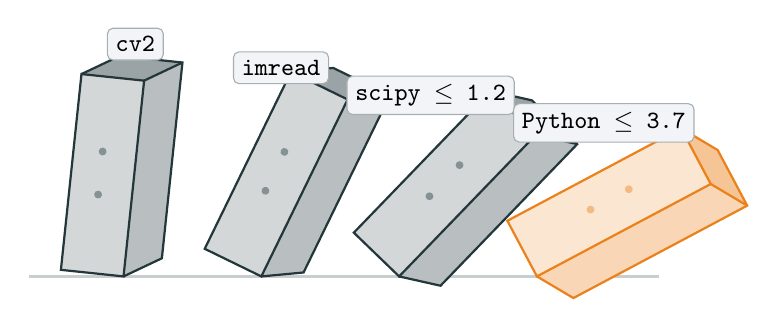
\begin{tikzpicture}[
  tag/.style={draw=navydeep!40, fill=softgray, rounded corners=2pt,
              font=\ttfamily\small, inner sep=3pt},
]
  % nền
  \draw[navydeep!25, line width=1pt] (-0.4,0) -- (7.6,0);
  % --- 4 quân domino mỏng, nghiêng tăng dần (té dây chuyền); quân cuối cam ---
  % mỗi quân xoay quanh chân phải (pivot) để giống đang đổ về phải
  \def\w{0.8}\def\h{2.5}\def\dx{0.46}\def\dy{0.28}
  \foreach \x/\rot/\col in {0/-6/navydeep, 1.75/-26/navydeep, 3.5/-44/navydeep, 5.25/-62/mLightBrown}{
    \begin{scope}[shift={(\x,0)}, rotate around={\rot:(\w,0)}]
      \fill[\col!32] (\w,0)--(\w+\dx,\dy)--(\w+\dx,\h+\dy)--(\w,\h)--cycle;          % side
      \fill[\col!46] (0,\h)--(\w,\h)--(\w+\dx,\h+\dy)--(\dx,\h+\dy)--cycle;          % top
      \fill[\col!20] (0,0) rectangle (\w,\h);                                        % front
      \fill[\col!55] (0.5*\w-0.03,0.62*\h) circle (0.05);                            % chấm domino
      \fill[\col!55] (0.5*\w-0.03,0.40*\h) circle (0.05);
      \draw[\col, line width=0.8pt] (0,0) rectangle (\w,\h);
      \draw[\col, line width=0.8pt] (0,\h)--(\dx,\h+\dy)--(\w+\dx,\h+\dy)--(\w+\dx,\dy)--(\w,0);
      \draw[\col, line width=0.8pt] (\w,\h)--(\w+\dx,\h+\dy);
    \end{scope}
  }
  % --- code tags phía trên, lệch theo hướng đổ ---
  \node[tag] at (0.95, 2.95) {cv2};
  \node[tag] at (2.8, 2.65) {imread};
  \node[tag] at (4.7, 2.30) {scipy $\le$ 1.2};
  \node[tag] at (6.9, 1.95) {Python $\le$ 3.7};
\end{tikzpicture}}
\caption{Hiệu ứng domino trong Dependency Hell}
\end{figure}
\end{columns}

\vspace{0.5em}
\begin{block}{Không gian tìm kiếm}
\footnotesize $\sim$\textcolor{alert}{\textbf{500K}} package PyPI $\times$ \textcolor{alert}{\textbf{chục}} phiên bản $\times$ \textcolor{alert}{\textbf{nhiều}} bản Python $\Rightarrow$ \emph{Bùng nổ tổ hợp}.
\end{block}
\end{frame}

\begin{frame}{Bùng nổ tổ hợp: Không gian tìm kiếm khổng lồ}
\begin{columns}[c]
% ===== LEFT: khối 3D không gian tìm kiếm =====
\column{0.55\textwidth}
\centering
\resizebox{\linewidth}{!}{%
\begin{tikzpicture}[font=\scriptsize,
  pkg/.style={draw=navydeep!60, fill=navydeep!8, rounded corners=2pt, font=\tiny\ttfamily, inner sep=2.5pt},
  ver/.style={circle, fill=navydeep!55, inner sep=1.3pt},
  edge/.style={navydeep!45, line width=0.4pt},
]
  % --- root: 1 import ---
  \node[draw=navydeep, fill=navydeep!12, rounded corners=3pt, font=\tiny\bfseries,
        inner sep=3pt, align=center] (root) at (-0.4,0) {1\\import};
  % --- level 1: packages (3 shown + "...500K") ---
  \node[pkg] (p1) at (1.9,1.65) {scipy};
  \node[pkg] (p2) at (1.9,0.45) {numpy};
  \node[pkg] (p3) at (1.9,-0.75) {cv2};
  \node[font=\scriptsize, navydeep!55] at (1.78,-1.65) {$\vdots$};
  \draw[edge] (root)--(p1); \draw[edge] (root)--(p2); \draw[edge] (root)--(p3);
  \draw[edge] (root)--(1.5,-1.6);
  \node[font=\tiny, navydeep!75] at (1.9,2.45) {$\sim$\textbf{500K} package};
  % --- level 2: ~10 versions / package (3 dots each) ---
  \foreach \yc in {1.65,0.45,-0.75}{
    \foreach \dy in {0.34,0,-0.34}{
      \pgfmathsetmacro\vy{\yc+\dy}
      \node[ver] at (3.35,\vy) {};
      \draw[edge] (2.5,\yc) -- (3.35,\vy);
    }
  }
  \node[font=\tiny, navydeep!75] at (3.35,2.45) {$\times\,\sim$\textbf{10} ver};
  % --- rays fanning into the front face of the 3D volume ---
  \foreach \yc in {1.65,0.45,-0.75}{
    \foreach \dy in {0.34,0,-0.34}{
      \pgfmathsetmacro\vy{\yc+\dy}
      \pgfmathsetmacro\ty{\vy*0.42-0.15}
      \draw[mLightBrown!35, line width=0.3pt] (3.5,\vy) -- (5.0,\ty);
  }}
  % --- 3D candidate-environment volume: cube PACKED with ~10^7 points (one is the solution) ---
  % point(i,j,k) = (5.0 + 0.40 i + 0.32 k, -1.25 + 0.40 j + 0.25 k); grid 6x6x5 = 180 dots.
  % depth (k) fades navy->faint and shrinks => clean 3D stacking, not a flat blob.
  % faint receding faces behind the cloud (kills the "hollow" look)
  \fill[navydeep!7]  (5.0,0.75) -- (7.0,0.75) -- (8.28,1.75) -- (6.28,1.75) -- cycle; % top
  \fill[navydeep!10] (7.0,-1.25) -- (7.0,0.75) -- (8.28,1.75) -- (8.28,-0.25) -- cycle; % right
  % hidden back edges (dashed, behind the cloud)
  \draw[navydeep!20, line width=0.4pt, dashed] (5.0,-1.25) -- (6.28,-0.25);
  \draw[navydeep!20, line width=0.4pt, dashed] (6.28,-0.25) -- (8.28,-0.25);
  \draw[navydeep!20, line width=0.4pt, dashed] (6.28,-0.25) -- (6.28,1.75);
  % the point cloud (drawn back -> front so nearer dots sit on top)
  \foreach \k in {4,3,2,1,0}{
    \pgfmathsetmacro\fr{\k/4}
    \pgfmathtruncatemacro\pp{84-\fr*56}
    \pgfmathsetmacro\rr{0.047-\fr*0.019}
    \foreach \i in {0,...,5}{ \foreach \j in {0,...,5}{
      \pgfmathsetmacro\sx{5.0+0.40*\i+0.32*\k}
      \pgfmathsetmacro\sy{-1.25+0.40*\j+0.25*\k}
      \fill[navydeep!\pp] (\sx,\sy) circle (\rr);
    }}
  }
  % visible bounding edges (thin frame around the cloud)
  \draw[navydeep!50, line width=0.55pt] (5.0,-1.25) -- (7.0,-1.25) -- (7.0,0.75) -- (5.0,0.75) -- cycle; % front
  \draw[navydeep!50, line width=0.55pt] (5.0,0.75) -- (6.28,1.75); % top-left depth edge (Python axis)
  \draw[navydeep!50, line width=0.55pt] (7.0,0.75) -- (8.28,1.75) -- (6.28,1.75); % top-right + back-top
  \draw[navydeep!50, line width=0.55pt] (7.0,-1.25) -- (8.28,-0.25) -- (8.28,1.75); % bottom-right + back-right
  % depth axis = the 3rd dimension that makes the space 3D (8 Python runtimes)
  \draw[->, navydeep!60, line width=0.5pt] (4.78,1.58) -- (5.40,1.18);
  \node[font=\tiny, navydeep!80, anchor=east] at (4.76,1.61) {$\times\,\sim$\textbf{8} Python};
  % --- the single valid solution: one point lifted out of the haystack ---
  \fill[white] (6.52,0.20) circle (0.135);
  \fill[mLightBrown] (6.52,0.20) circle (0.085);
  \draw[mLightBrown!85!black, line width=0.8pt] (6.52,0.20) circle (0.175);
  \draw[mLightBrown!35, line width=0.6pt] (6.52,0.20) circle (0.285);
  \draw[mLightBrown!85!black, line width=0.5pt] (6.52,0.37) -- (6.52,1.97);
  \node[font=\tiny\bfseries, mLightBrown!85!black, anchor=south] at (6.52,1.95) {1 lời giải};
  % --- climax ---
  \node[font=\footnotesize\bfseries, alert] at (6.4,-1.8) {$\approx 10^{7}$ tổ hợp};
\end{tikzpicture}}

% ===== RIGHT: giải thích =====
\column{0.45\textwidth}
\footnotesize
\textbf{\color{navydeep}Mỗi \texttt{import} phải khớp đồng thời:}
\begin{itemize}\setlength{\itemsep}{2pt}
  \item \textbf{Package}: đúng tên pip\\{\scriptsize\color{gray}(vd \texttt{cv2} $\to$ \texttt{opencv-python})}
  \item \textbf{Version}: 1 trong $\sim$10 bản thư viện
  \item \textbf{Python}: 1 trong $\sim$8 runtime
\end{itemize}

\vspace{0.6em}
{\scriptsize\color{mDarkTeal}$\Rightarrow$ Không thể thử hết bằng tay, cần solver/agent để \textbf{tỉa không gian}.}
\end{columns}
\end{frame}

% --- Datasets (HG2.9K + GitChameleon) ---
\begin{frame}{Datasets}
\vspace{0.6em}
\centering
\begin{tikzpicture}[
  dcard/.style={rounded corners=8pt, line width=1pt,
                text width=5.9cm, inner sep=11pt, align=left, anchor=north},
  badge/.style={rounded corners=3pt, inner sep=2.5pt, font=\tiny\bfseries, text=white},
]
% --- HG2.9K ---
\node[dcard, draw=navydeep!45, fill=navydeep!4] (hg) at (-3.7,3.05) {%
  {\Large\bfseries\color{navydeep} HG2.9K}\hfill\colorbox{navydeep}{\color{white}\tiny\bfseries In-distribution}
  \vspace{4pt}\textcolor{navydeep!30}{\rule{\linewidth}{0.6pt}}\vspace{5pt}
  \scriptsize
  {\bfseries\color{mLightBrown}Quy mô}\\ 2.891 gist Python ``khó'' (hard subset của Gistable, ICSME'18).\\[4pt]
  {\bfseries\color{mLightBrown}Đặc điểm}\\ File đơn lẻ, không \texttt{requirements}; lẫn Python 2/3; thư viện khoa học cũ; phụ thuộc native C/C++.\\[4pt]
  {\bfseries\color{mLightBrown}Nhiệm vụ}\\ Khôi phục môi trường để mọi \texttt{import} chạy được trong Docker.\\[4pt]
  {\bfseries\color{mLightBrown}Đánh giá}\\ Pass rate (build + import OK).
};
% --- GitChameleon ---
\node[dcard, draw=success!55!black!45, fill=success!55!black!4] (gc) at (3.7,3.05) {%
  {\Large\bfseries\color{navydeep} GitChameleon}\hfill\colorbox{success!55!black}{\color{white}\tiny\bfseries Out-of-distribution}
  \vspace{4pt}\textcolor{success!40!black!40}{\rule{\linewidth}{0.6pt}}\vspace{5pt}
  \scriptsize
  {\bfseries\color{mLightBrown}Quy mô}\\ 328 snippet Python, kèm \textbf{unit test ẩn} + version ground-truth.\\[4pt]
  {\bfseries\color{mLightBrown}Đặc điểm}\\ Xoáy vào \textit{breaking changes} giữa các version thư viện (phải dùng đúng API của đúng bản).\\[4pt]
  {\bfseries\color{mLightBrown}Nhiệm vụ}\\ Chọn \textbf{đúng phiên bản} để snippet vừa chạy vừa \textbf{pass unit test}.\\[4pt]
  {\bfseries\color{mLightBrown}Đánh giá}\\ Pass rate theo unit test (đúng ngữ nghĩa).
};
\end{tikzpicture}

\vspace{0.3em}
\centering\tiny\color{gray}
\textit{HG2.9K: hard subset 2891 gist từ Gistable (Horton \& Parnin, ICSME'18), gold standard cho dependency resolution. GitChameleon: 328 snippet có unit test, re-frame từ GitChameleon 2.0 (arXiv:2507.12367) để đánh giá khả năng tổng quát hóa (OOD).}
\end{frame}

% --- Related Work 1/2: 3 hướng tiếp cận (concept, không nêu tên method) ---
\begin{frame}{Related Work: 3 hướng tiếp cận}
\centering
\begin{tikzpicture}[font=\scriptsize,
  rwcard/.style={rounded corners=6pt, line width=1pt, text width=3.5cm,
                 inner sep=9pt, align=left, anchor=north, minimum height=5.3cm},
  rwnum/.style={circle, text=white, font=\bfseries\footnotesize, inner sep=2.6pt},
]
  % ---- 1. Knowledge Graph (navy) ----
  \node[rwcard, draw=navydeep!45, fill=navydeep!4] (c1) at (-3.85,3.0) {%
    \hspace*{0.62cm}\textbf{\normalsize\color{navydeep}Knowledge Graph}\\[3pt]
    \textcolor{navydeep!25}{\rule{\linewidth}{0.5pt}}\\[4pt]
    \textbf{Ý tưởng:} encode quan hệ module--version thành đồ thị tri thức (Libraries.io, PyPI); truy vấn để suy dependency tương thích.\\[5pt]
    {\color{success!50!black}\cmark\ \textbf{Ưu:}} cấu trúc rõ, deterministic, dễ giải thích.\\[5pt]
    {\color{alert}\xmark\ \textbf{Hạn chế:}} DB lỗi thời nhanh, gãy khi registry đổi schema.};
  \node[rwnum, fill=navydeep] at (-5.35,2.55) {1};
  % ---- 2. Regex / Log-parsing (gold; orange reserved for "ours") ----
  \node[rwcard, draw=cSoft!75!black, fill=cSoft!14] (c2) at (0,3.0) {%
    \hspace*{0.62cm}\textbf{\normalsize\color{cSoft!55!black}Regex / Log-parsing}\\[3pt]
    \textcolor{cSoft!45}{\rule{\linewidth}{0.5pt}}\\[4pt]
    \textbf{Ý tưởng:} parse error log bằng regex để suy missing dependency, patch môi trường rồi build lại.\\[5pt]
    {\color{success!50!black}\cmark\ \textbf{Ưu:}} nhẹ, runtime-driven, không cần DB.\\[5pt]
    {\color{alert}\xmark\ \textbf{Hạn chế:}} \emph{brittle}, log đổi định dạng (Python/pip update) là parser vỡ.};
  \node[rwnum, fill=cSoft!72!black] at (-1.5,2.55) {2};
  % ---- 3. LLM + RAG (teal) ----
  \node[rwcard, draw=success!55!black!45, fill=success!55!black!5] (c3) at (3.85,3.0) {%
    \hspace*{0.62cm}\textbf{\normalsize\color{success!45!black}LLM + RAG}\\[3pt]
    \textcolor{success!40!black!30}{\rule{\linewidth}{0.5pt}}\\[4pt]
    \textbf{Ý tưởng:} LLM sinh giả thuyết, RAG cấp PyPI metadata, Docker build phản hồi, lặp lại.\\[5pt]
    {\color{success!50!black}\cmark\ \textbf{Ưu:}} adaptive, không cần hạ tầng tĩnh, tận dụng pretrain.\\[5pt]
    {\color{alert}\xmark\ \textbf{Hạn chế:}} thử-sai mù, thất bại \emph{không thành tri thức} để tỉa không gian.};
  \node[rwnum, fill=success!45!black] at (2.35,2.55) {3};
\end{tikzpicture}

\vspace{0.5em}
{\centering\footnotesize\textcolor{mDarkTeal}{\textbf{Khoảng trống:} chưa phương pháp nào \emph{học từ thất bại} để thu hẹp không gian tìm kiếm một cách hệ thống.}\par}
\end{frame}

% --- Related Work 2/2: Bảng tổng hợp method × venue × hạn chế + timeline viz ---
\begin{frame}{Related Work: Tổng hợp các phương pháp}
\begin{columns}[c,onlytextwidth]
\column{0.55\textwidth}
\tiny
\setlength{\tabcolsep}{3pt}
\renewcommand{\arraystretch}{1.15}
\begin{tabular}{@{}l l l l@{}}
  \toprule
  \textbf{Method} & \textbf{Venue} & \textbf{Approach} & \textbf{Key limitation} \\
  \midrule
  \rowcolor{navydeep!8}
  PyEGo              & ICSE'22  & KG + SMT (Z3)           & DB stale \\
  \rowcolor{navydeep!8}
  ReadPyE            & TSE'24   & KG + README naming      & DB drift \\
  \midrule
  \rowcolor{cSoft!18}
  PyDFix             & ISSTA'21 & Regex log-parse         & Format brittle \\
  \midrule
  \rowcolor{cInferL}
  GPT-4o / o1        & 2024     & Closed LLM (direct)     & Closed, expensive \\
  \rowcolor{cInferL}
  GPT-4.1 + RAG      & 2025     & Closed LLM + RAG        & Closed, no constraint \\
  \midrule
  \rowcolor{success!10}
  PLLM               & arXiv'25 & Open LLM + RAG iter.    & Blind trial-and-error \\
  \rowcolor{success!10}
  SMT-LLM            & FSE'26   & Z3 SMT + LLM imput.     & Static metadata only \\
  \bottomrule
\end{tabular}

\vspace{0.5em}
\tiny
\textcolor{navydeep}{$\blacksquare$} KG \quad
\textcolor{cSoft!65!black}{$\blacksquare$} Log-parse \quad
\textcolor{cInfer}{$\blacksquare$} Closed LLM \quad
\textcolor{success!50!black}{$\blacksquare$} Open LLM+RAG

\column{0.45\textwidth}
\centering
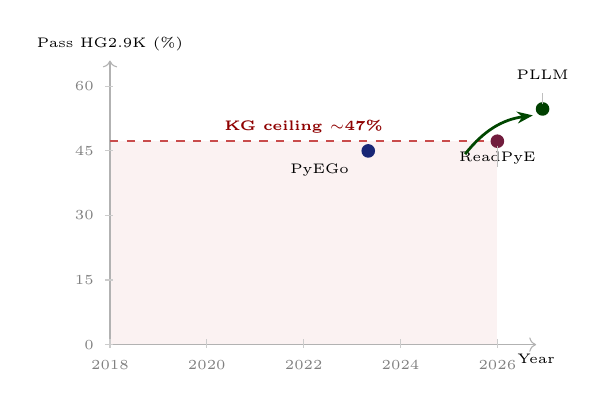
\begin{tikzpicture}[scale=0.82]
  \def\xmin{0}\def\xmax{6.3}\def\ymin{0}\def\ymax{4.2}
  % KG-era ceiling zone (region under ~47% where KG methods stayed stuck)
  \fill[alert!5] (\xmin,\ymin) rectangle (6.0, 3.15);
  % Axes
  \draw[->, gray!60] (\xmin,\ymin) -- (\xmax+0.3, \ymin) node[below, font=\tiny, black]{Year};
  \draw[->, gray!60] (\xmin,\ymin) -- (\xmin, \ymax+0.2)
    node[above, font=\tiny, black]{Pass HG2.9K (\%)};
  % Y ticks (1 unit = 15%)
  \foreach \y/\v in {0/0, 1/15, 2/30, 3/45, 4/60} {
    \draw[gray!40] (\xmin-0.08, \y) -- (\xmin+0.05, \y);
    \node[font=\tiny, gray, anchor=east] at (\xmin-0.1, \y) {\v};
  }
  % X ticks (1 unit = 1 year, base 2018)
  \foreach \x/\v in {0/2018, 1.5/2020, 3/2022, 4.5/2024, 6/2026} {
    \draw[gray!40] (\x, \ymin-0.05) -- (\x, \ymin+0.08);
    \node[font=\tiny, gray, anchor=north] at (\x, \ymin-0.1) {\v};
  }
  % KG plateau line at 47% (y=3.15) -- extend only through KG era (ReadPyE 2024)
  \draw[dashed, alert!70, thick] (\xmin, 3.15) -- (6.0, 3.15);
  \node[font=\tiny\bfseries, alert!80!black, anchor=south, fill=white, inner sep=1.5pt]
    at (3.0, 3.20) {KG ceiling $\sim$47\%};

  % Data points  ---  each method its own color
  % PyEGo (2022, 45.0%) -> (4, 3.0)
  \fill[mDarkTeal!70!blue] (4, 3.0) circle (3pt);
  \node[font=\tiny, anchor=east] at (3.85, 2.7) {PyEGo};
  % ReadPyE (2024, 47.2%) -> (6, 3.15)
  \fill[navydeep!50!purple] (6, 3.15) circle (3pt);
  \node[font=\tiny, anchor=south] at (6, 2.65) {ReadPyE};
  \draw[gray!50, very thin] (6, 3.08) -- (6, 2.75);
  % PLLM (2025, 54.8% = 1583/2891, 10-run union) -> (6.7, 3.65)
  \fill[success!50!black] (6.7, 3.65) circle (3pt);
  \node[font=\tiny, anchor=south] at (6.7, 3.95) {PLLM};
  \draw[gray!50, very thin] (6.7, 3.72) -- (6.7, 3.9);
  % breakthrough: LLM paradigm crosses the KG ceiling
  \draw[-{Stealth[length=2mm]}, success!55!black, line width=1pt]
    (5.5, 2.95) to[bend left=22] (6.55, 3.55);
\end{tikzpicture}

\vspace{0.4em}
\scriptsize \textcolor{mDarkTeal}{KG-era \emph{ceiling $\sim$47\%} trên HG2.9K; PLLM (LLM paradigm) phá vỡ lên $\sim$55\%.}\\
{\tiny\color{gray} Nguồn: \textit{Raiders of the Lost Dependency} (arXiv:2501.16191), Table 1: PyEGo 45.0\% (1302/2891), ReadPyE 47.2\% (1365/2891), PLLM 54.8\% (1583/2891, 10-run union). Trong harness của nhóm, PLLM single-run = 44.8\% (số dùng ở bảng so sánh).}
\end{columns}
\end{frame}

% ============================================================
\section{MEMRES}
% ============================================================

\begin{frame}{MEMRES: Lookup-First, LLM-Last}

\vspace{0.5em}
\begin{columns}[T]
\column{0.66\textwidth}
\centering
\href{https://arxiv.org/abs/2604.16941}{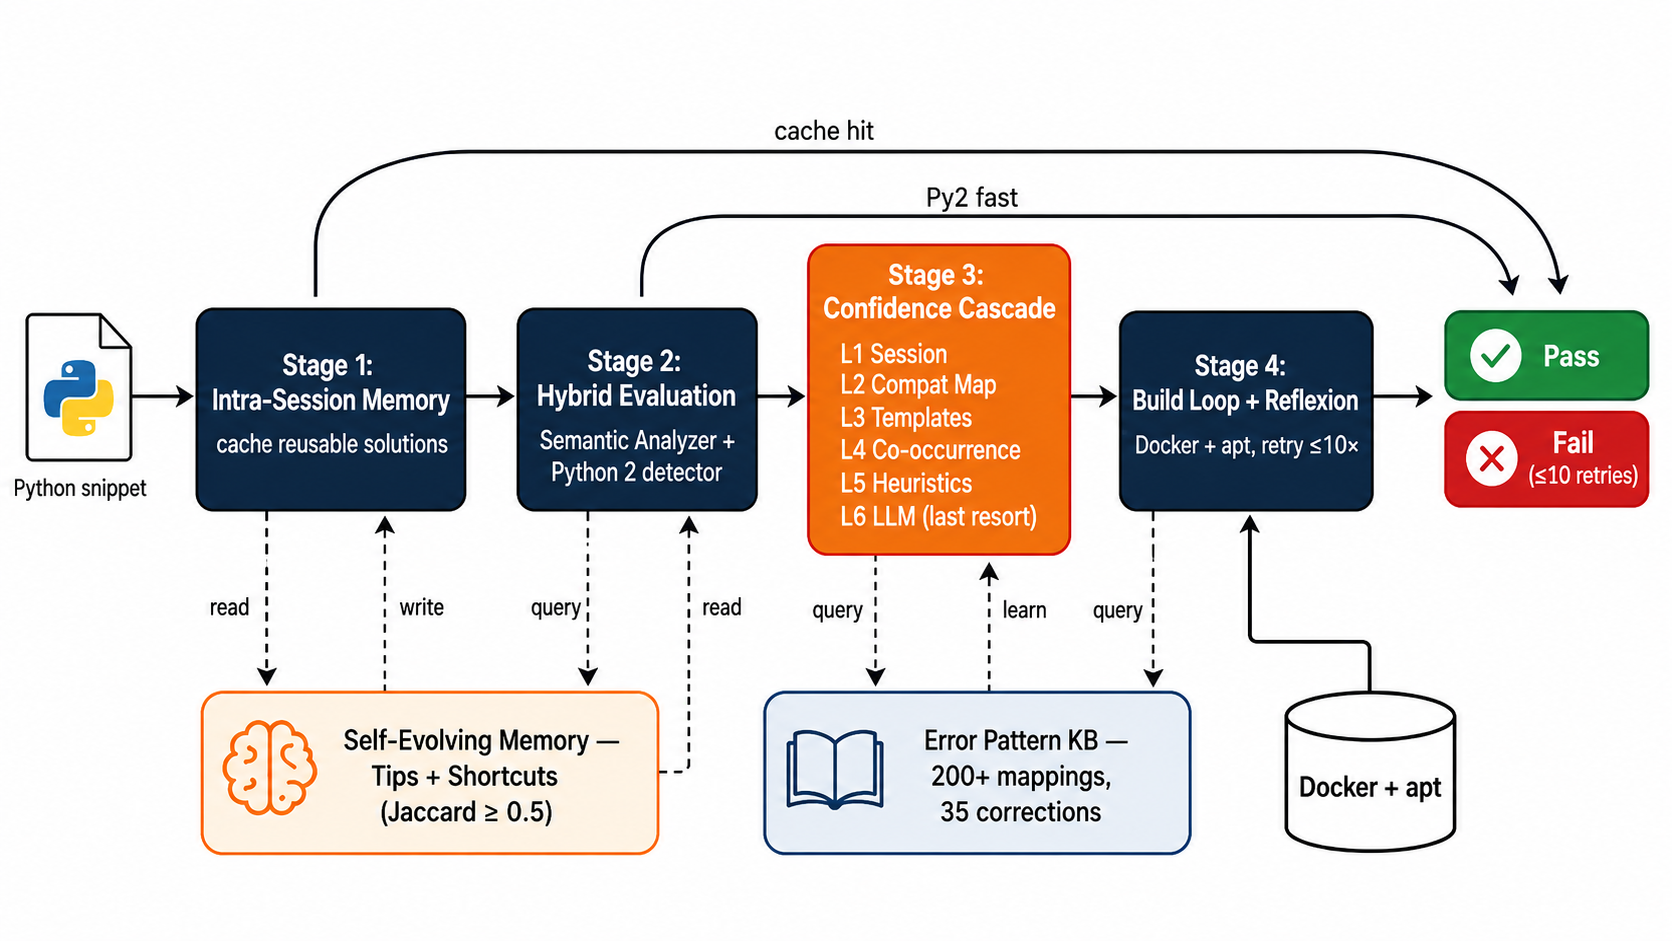
\includegraphics[width=\linewidth]{memres-pipeline.png}}

\vspace{0.3em}
{\tiny\color{gray}\textit{4 stages + 2 fast paths (cache hit, Py2 fast); 2 memory stores feed back vào pipeline.}\\
Figure: paper gốc MEMRES, \href{https://arxiv.org/abs/2604.16941}{\textcolor{mLightBrown}{arXiv:2604.16941}}}

\column{0.32\textwidth}
\centering
\vspace{0.5em}
{\scriptsize\textbf{\color{navydeep}Pass rate (\%)}}
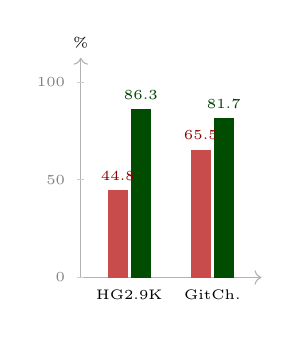
\begin{tikzpicture}[scale=0.62]
  \draw[->, gray!60] (0,0) -- (3.7,0);
  \draw[->, gray!60] (0,0) -- (0,4.5) node[above, font=\tiny, black]{\%};
  \foreach \y/\v in {0/0, 2/50, 4/100} {
    \draw[gray!40] (-0.08,\y) -- (0.06,\y);
    \node[font=\tiny, gray, anchor=east] at (-0.12,\y) {\v};
  }
  \def\bw{0.42}
  % --- HG2.9K group: PLLM 44.8 vs MEMRES 86.3 (1 unit = 25%) ---
  \fill[alert!70]         (0.55,0)            rectangle ++(\bw, 1.792);
  \fill[success!60!black] (0.55+\bw+0.05,0)   rectangle ++(\bw, 3.452);
  \node[font=\tiny, anchor=north] at (0.55+\bw+0.025, -0.06) {HG2.9K};
  \node[font=\tiny, anchor=south, color=alert!80!black]   at (0.55+\bw/2, 1.792) {44.8};
  \node[font=\tiny, anchor=south, color=success!50!black] at (0.55+\bw+0.05+\bw/2, 3.452) {86.3};
  % --- GitChameleon group: PLLM 65.5 vs MEMRES 81.7 ---
  \fill[alert!70]         (2.25,0)            rectangle ++(\bw, 2.62);
  \fill[success!60!black] (2.25+\bw+0.05,0)   rectangle ++(\bw, 3.268);
  \node[font=\tiny, anchor=north] at (2.25+\bw+0.025, -0.06) {GitCh.};
  \node[font=\tiny, anchor=south, color=alert!80!black]   at (2.25+\bw/2, 2.62) {65.5};
  \node[font=\tiny, anchor=south, color=success!50!black] at (2.25+\bw+0.05+\bw/2, 3.268) {81.7};
\end{tikzpicture}

\vspace{0.1em}
{\tiny
\textcolor{alert}{$\blacksquare$} PLLM \quad
\textcolor{success!50!black}{$\blacksquare$} \textbf{MEMRES}}

\vspace{0.4em}
\scriptsize
\textbf{\color{navydeep}Ý tưởng:} cascade rẻ trước $\to$ đắt sau; memory tích lũy giữa retries.
\end{columns}

\vspace{0.3em}
\centering\footnotesize\color{mDarkTeal}
MEMRES = \emph{Memory-augmented retry}: cứu được nhiều lỗi, nhưng chưa biến thất bại thành \emph{ràng buộc logic} để tỉa không gian.
\end{frame}

\begin{frame}{Từ MEMRES đến CGAR: Vá Đúng 3 Lỗ Hổng}
\centering
\begin{tikzpicture}[
  font=\scriptsize,
  gaptext/.style={anchor=west, text width=4.35cm, align=left, inner sep=1pt},
  fixtext/.style={anchor=west, text width=4.5cm, align=left, inner sep=1pt},
  numb/.style={circle, fill=mDarkTeal, text=white, font=\bfseries\scriptsize, inner sep=1.7pt},
  va/.style={-{Stealth[length=2.6mm]}, line width=1.5pt, mLightBrown},
]
  \def\xg{-5.7}\def\xaa{-1.05}\def\xbb{0.25}\def\xf{0.7}
  % 3 rows: MEMRES gap --vá--> CGAR component
  \foreach \y/\n/\gt/\gd/\ft/\fd in {%
      2.5/1/{12.8\% bí đường}/{API removed / source-only, build kẹt 3 phút}/{Analyzer Agent}/{parse log $\to$ constraint},%
      1.3/2/{Chi phí lỗi cao}/{335s/snippet, fail tốn gần trọn budget}/{wheel\_filter()}/{chỉ thử bản có wheel},%
      0.1/3/{Không tỉa không gian}/{Docker error = blackbox, không thành ràng buộc}/{3-tier constraints}/{HARD / SOFT / UPPER}}{
    \node[numb] at (-6.15,\y) {\n};
    \node[gaptext] at (\xg,\y) {{\color{alert}\xmark\ \textbf{\gt}}\\[1pt]{\tiny\color{gray}\gd}};
    \draw[va] (\xaa,\y) -- (\xbb,\y);
    \node[font=\tiny\bfseries, mLightBrown!85!black] at ({(\xaa+\xbb)/2},\y+0.23) {vá};
    \node[fixtext] at (\xf,\y) {{\color{success!45!black}\cmark\ \textbf{\ft}}\\[1pt]{\tiny\color{gray}\fd}};
  }
  % row separators
  \draw[gray!22, line width=0.5pt] (-6.4,1.9) -- (5.45,1.9);
  \draw[gray!22, line width=0.5pt] (-6.4,0.7) -- (5.45,0.7);
  % foundation: CGAR (de-boxed, thin orange rule)
  \draw[mLightBrown!55, line width=1pt] (-6.4,-0.62) -- (5.45,-0.62);
  \node[align=center] at (-0.475,-1.2) {%
    \textbf{\normalsize\color{mDarkTeal}CGAR: Constraint-Guided Agentic Resolution}\\[3pt]
    \textcolor{alert}{\textbf{LLM đoán mò}}$\;\xrightarrow{\;\text{paradigm shift}\;}\;$\textcolor{success!45!black}{\textbf{Multi-Agent + Constraint Acquisition}} (ràng buộc \emph{học} từ verifier)};
\end{tikzpicture}

\vspace{0.5em}
{\centering\footnotesize Mỗi lỗ hổng MEMRES $\to$ một thành phần CGAR: \textbf{vá có chủ đích}.\par}
\end{frame}

% ============================================================
\section{CGAR: Multi-Agent Architecture}
% ============================================================

\begin{frame}{CGAR: Tổng quan 3 Agent}
    \begin{figure}
        \centering
        \href{https://chatgpt.com/share/6a2a3c91-5640-83ec-8761-25876b30abe3}{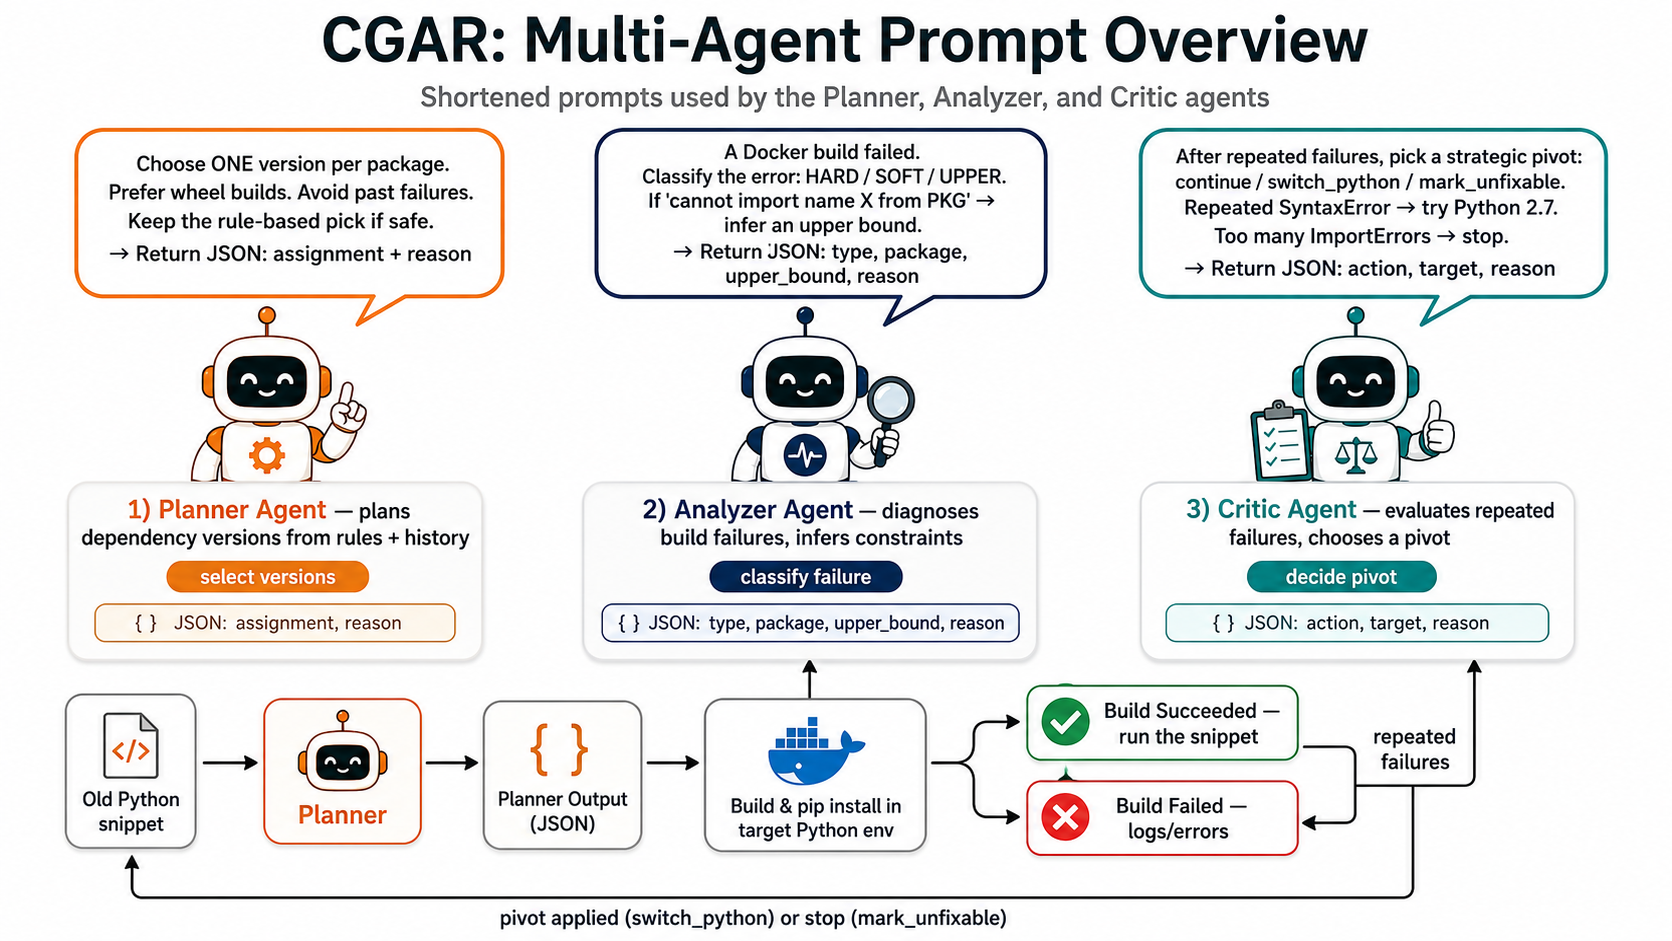
\includegraphics[height=0.74\textheight]{cgar-overview.png}}
    \end{figure}
    \vspace{-0.5em}
    \centering\footnotesize\color{mDarkTeal}
    3 LLM agent (Planner / Analyzer / Critic) + Docker build loop; chi tiết prompt ở phần Backup.\\
    {\tiny\color{gray}Minh họa AI, \href{https://chatgpt.com/share/6a2a3c91-5640-83ec-8761-25876b30abe3}{\textcolor{mLightBrown}{ChatGPT prompt}}}
\end{frame}

\begin{frame}{CGAR: Multi-Agent Loop}

\centering
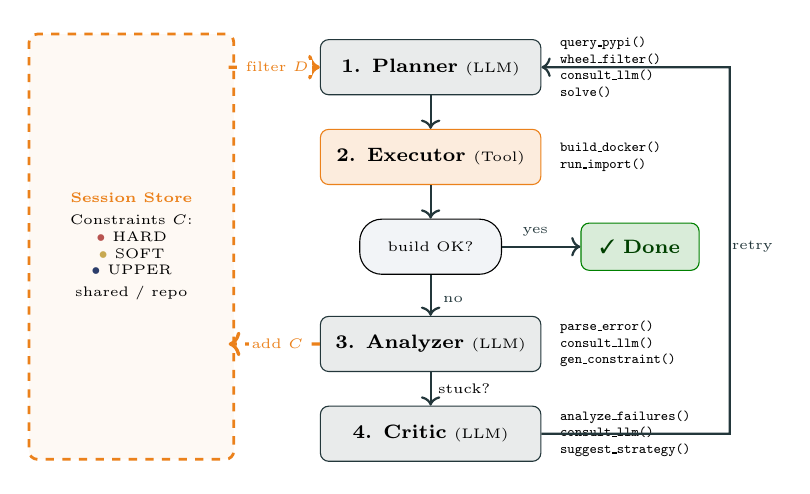
\begin{tikzpicture}[scale=0.95]
  % Styles
  \tikzstyle{llmnode}=[draw=mDarkTeal, fill=mDarkTeal!10, rounded corners=3pt,
                       minimum width=2.8cm, minimum height=0.7cm, align=center, font=\scriptsize]
  \tikzstyle{toolnode}=[draw=mLightBrown, fill=mLightBrown!15, rounded corners=3pt,
                        minimum width=2.8cm, minimum height=0.7cm, align=center, font=\scriptsize]
  \tikzstyle{decnode}=[draw, fill=softgray, rounded corners=8pt,
                       minimum width=1.8cm, minimum height=0.7cm, font=\tiny, align=center]
  \tikzstyle{donenode}=[draw=success, fill=success!15, rounded corners=3pt,
                        minimum width=1.5cm, minimum height=0.6cm, font=\scriptsize\bfseries]
  \tikzstyle{storenode}=[draw=mLightBrown, fill=mLightBrown!5, rounded corners=3pt,
                         dashed, line width=1pt, align=center, font=\tiny,
                         minimum width=2.6cm, minimum height=5.4cm]
  \tikzstyle{toolslabel}=[font=\tiny\ttfamily, align=left]
  \tikzstyle{arrline}=[->, thick, color=mDarkTeal]
  \tikzstyle{backline}=[->, very thick, dashed, color=mLightBrown]

  % Session Store (left)
  \node[storenode] (store) at (-3.5, 0)
    {\textbf{\color{mLightBrown}Session Store}\\[2pt]
     Constraints $C$:\\
     \textcolor{cHard}{$\bullet$} HARD\\
     \textcolor{cSoft}{$\bullet$} SOFT\\
     \textcolor{cInfer}{$\bullet$} UPPER\\[2pt]
     {\tiny shared / repo}};

  % Vertical chain of agents (shifted left to center the diagram)
  \node[llmnode]  (planner) at (0.5,  2.4) {\textbf{1. Planner} \tiny(LLM)};
  \node[toolnode] (exec)    at (0.5,  1.2) {\textbf{2. Executor} \tiny(Tool)};
  \node[decnode]  (dec)     at (0.5,  0.0) {build OK?};
  \node[donenode] (done)    at (3.3,  0.0) {\color{success!50!black}\cmark\ Done};
  \node[llmnode]  (ana)     at (0.5, -1.3) {\textbf{3. Analyzer} \tiny(LLM)};
  \node[llmnode]  (crit)    at (0.5, -2.5) {\textbf{4. Critic} \tiny(LLM)};

  % Tool annotations
  \node[toolslabel, anchor=west] at (2.1, 2.4)  {query\_pypi()\\wheel\_filter()\\\textbf{consult\_llm()}\\solve()};
  \node[toolslabel, anchor=west] at (2.1, 1.2)  {build\_docker()\\run\_import()};
  \node[toolslabel, anchor=west] at (2.1, -1.3) {parse\_error()\\\textbf{consult\_llm()}\\gen\_constraint()};
  \node[toolslabel, anchor=west] at (2.1, -2.5) {analyze\_failures()\\\textbf{consult\_llm()}\\suggest\_strategy()};

  % Main flow
  \draw[arrline] (planner) -- (exec);
  \draw[arrline] (exec)    -- (dec);
  \draw[arrline] (dec)     -- (done);
  \draw[arrline] (dec)     -- (ana);
  \draw[arrline] (ana)     -- (crit);

  % Edge labels
  \node[font=\tiny, color=mDarkTeal] at (1.9, 0.2) {yes};
  \node[font=\tiny, color=mDarkTeal] at (0.8, -0.7) {no};
  \node[font=\tiny] at (0.95, -1.9) {stuck?};

  % Loop back
  \draw[arrline] (crit.east) -- (4.5, -2.5) -- (4.5, 2.4) -- (planner.east);
  \node[font=\tiny, color=mDarkTeal] at (4.8, 0) {retry};

  % Memory write (ana -> store)
  \draw[backline] (ana.west) -- (-2.2, -1.3);
  \node[font=\tiny, color=mLightBrown, fill=white, inner sep=1pt] at (-1.55, -1.3) {add $C$};

  % Memory read (store -> planner)
  \draw[backline] (-2.2, 2.4) -- (planner.west);
  \node[font=\tiny, color=mLightBrown, fill=white, inner sep=1pt] at (-1.55, 2.4) {filter $D$};
\end{tikzpicture}

\vspace{0.4em}
\centering\scriptsize
\textbf{Flow}: Planner $\to$ Executor $\to$ (OK?) $\to$ Analyzer ghi constraint vào Store $\to$ vòng kế đọc Store trước khi chọn.

\vspace{0.3em}
\centering\footnotesize\color{mDarkTeal}
Build thất bại không phí: mỗi lần fail $\to$ +1 constraint $\to$ Planner kế tiếp né cả vùng, điều MEMRES không có.
\end{frame}

% ─── CGAR: miền giá trị D đến từ đâu (PyPI filter, reveal từng bước) ───
\begin{frame}{CGAR: Miền giá trị $D$ đến từ đâu? (lọc trực tuyến từ PyPI)}
\centering
\vspace{0.1em}
\begin{tikzpicture}[font=\scriptsize,
  num/.style={circle, fill=navydeep, text=white, font=\bfseries\tiny, inner sep=2pt},
  snip/.style={draw=gray!45, fill=softgray, rounded corners=3pt, font=\ttfamily\scriptsize, inner sep=4pt, align=left},
  mapb/.style={rounded corners=3pt, draw=navydeep!50, fill=navydeep!8, inner sep=4pt, align=left, text width=3.7cm, font=\tiny},
  getb/.style={rounded corners=3pt, draw=alert!70, fill=alert!8, line width=1pt, inner sep=4pt, align=left, text width=3.7cm, font=\tiny\ttfamily},
  filt/.style={rounded corners=3pt, draw=cUpper!70, fill=cUpper!12, inner sep=4pt, align=left, text width=3.7cm, font=\tiny},
  card/.style={draw=navydeep!50, fill=navydeep!4, rounded corners=6pt, line width=1pt, inner sep=7pt, align=left, text width=4.7cm},
  ar/.style={-{Stealth[length=2mm]}, line width=0.9pt, navydeep!60},
  arh/.style={-{Stealth[length=2mm]}, line width=0.9pt, alert!70},
]
  % ---- LEFT: numbered pipeline ----
  \node<1->[num] at (-6.5,2.5) {1};
  \node<1->[snip] (s1) at (-4.7,2.5) {from scipy.misc import imread\\ {\scriptsize\rmfamily target Python $\pi=3.7$}};

  \node<2->[num] at (-6.5,1.4) {2};
  \node<2->[mapb] (s2) at (-4.7,1.4) {\textbf{import $\to$ pip} {\tiny(static map)}\\ \texttt{scipy.misc}$\to$\texttt{scipy}; \texttt{numpy} = dep của scipy};
  \draw<2->[ar] (s1.south) -- (s2.north);

  \node<3->[num,fill=alert] at (-6.5,0.25) {3};
  \node<3->[getb] (s3) at (-4.7,0.25) {GET pypi.org/pypi/\textbf{scipy}/json\\ GET pypi.org/pypi/\textbf{numpy}/json\\ {\rmfamily\tiny\color{alert!60!black} HTTP trực tiếp, KHÔNG LLM}};
  \draw<3->[ar] (s2.south) -- (s3.north);

  \node<4->[num] at (-6.5,-0.95) {4};
  \node<4->[filt] (s4) at (-4.7,-0.95) {\textbf{Lọc} mỗi version: giữ nếu\\ \texttt{requires\_python}$\,\models\pi\;\wedge\;$\texttt{has\_wheel}\\ {\tiny bỏ pre/post/dev release}};
  \draw<4->[ar] (s3.south) -- (s4.north);

  \node<5->[num] at (-6.5,-2.1) {5};
  \node<5->[filt] (s5) at (-4.7,-2.1) {\textbf{Sort} wheel-first, semver $\downarrow$ $\to$ lấy \textbf{top-8}/gói};
  \draw<5->[ar] (s4.south) -- (s5.north);

  % ---- RIGHT: artifacts ----
  \node<3->[card] (json) at (2.8,1.05)
    {{\bfseries\color{navydeep}PyPI JSON (rút gọn)}\\[1pt]\textcolor{navydeep!30}{\rule{\linewidth}{0.5pt}}\\[2pt]
     {\ttfamily\tiny releases:}\\
     {\ttfamily\tiny\quad 1.7.3 $\to$ req\_py $\geq$3.7, wheel cp37-manylinux \cmark}\\
     {\ttfamily\tiny\quad 1.2.3 $\to$ req\_py py3.7, wheel cp37 \cmark}\\
     {\rmfamily\tiny\quad\ldots\ $\sim$60 bản phát hành trên PyPI}};
  \draw<3->[arh, dashed] (s3.east) to[bend left=12] (json.west);

  \node<5->[card] (dom) at (2.8,-1.6)
    {{\bfseries\color{cUpper!85!black}Domain $D$ (đầu vào solver)}\\[1pt]\textcolor{cUpper!40}{\rule{\linewidth}{0.5pt}}\\[2pt]
     {\ttfamily\tiny $D$(scipy)$=$[1.7.3, 1.7.2, 1.7.1, \ldots]} {\rmfamily\tiny ·8}\\
     {\ttfamily\tiny $D$(numpy)$=$[1.21.6, 1.21.5, \ldots]} {\rmfamily\tiny ·8}\\
     {\rmfamily\tiny\color{gray}(mỗi ứng viên \cmark wheel \cmark py$\geq$3.7)}\\[2pt]
     {\rmfamily\tiny\color{alert}$\approx\!10^{7}$ (không gian gốc, toàn cục) $\to$ $\le$8 ứng viên/gói}};
  \draw<5->[ar] (s5.east) to[bend right=12] (dom.west);
\end{tikzpicture}

\vspace{0.2em}
\onslide<6->{{\centering\footnotesize\color{mDarkTeal} $D$ = top-8 ứng viên \textbf{có wheel}, hợp $\pi$, lọc từ \textbf{PyPI trực tiếp} (reducer xác định, \textbf{0 LLM}); là đầu vào cho solver \& ràng buộc học được.\par}}
\end{frame}

\begin{frame}{CGAR: Tích lũy ràng buộc (ví dụ)}
\centering
\vspace{0.3em}
\begin{tikzpicture}[font=\scriptsize,
  pill/.style={rounded corners=3pt, draw=navydeep!50, fill=navydeep!8, inner sep=4pt, font=\ttfamily\scriptsize},
  dock/.style={rounded corners=3pt, draw=cUpper!60, fill=cUpper!12, inner sep=4pt, font=\tiny},
  fail/.style={rounded corners=3pt, draw=alert!60, fill=alert!8, inner sep=4pt, align=left, text width=2.7cm, font=\tiny},
  okb/.style={rounded corners=3pt, draw=success!60!black, fill=success!14, inner sep=5pt, font=\scriptsize\bfseries, text=success!45!black},
  cons/.style={rounded corners=3pt, draw=cUpper, fill=cUpper!14, inner sep=4pt, align=left, text width=3.3cm, font=\tiny},
  ar/.style={-{Stealth[length=2mm]}, line width=0.9pt, navydeep!60},
]
  % snippet
  \node[draw=gray!45, fill=softgray, rounded corners=3pt, font=\ttfamily\scriptsize, inner sep=5pt] (snip) at (-3.4,3.4)
    {from scipy.misc import imread};
  % ---- Bước 1 (fail) ----
  \node[circle, fill=alert, text=white, font=\bfseries\tiny, inner sep=2pt] at (-6.25,2.25) {1};
  \node[pill] (a1) at (-5.1,2.25) {scipy 1.7.3};
  \node[dock] (d1) at (-3.4,2.25) {Docker build};
  \node[fail] (f1) at (-1.0,2.25) {\xmark\ ImportError: cannot import name \texttt{imread}};
  \draw[ar] (a1)--(d1); \draw[ar] (d1)--(f1);
  % analyzer -> constraint
  \node[cons] (c1) at (-3.2,1.15) {Analyzer: \textbf{scipy $<$ 1.3}  {\color{cUpper}[UPPER]}};
  \draw[ar, mLightBrown] (f1.south) |- (c1.east);
  % ---- Bước 2 (pass) ----
  \node[circle, fill=success!55!black, text=white, font=\bfseries\tiny, inner sep=2pt] at (-6.25,-0.05) {2};
  \node[pill] (a2) at (-5.1,-0.05) {scipy 1.2.3};
  \node[font=\tiny, gray, anchor=north] at (-5.1,-0.45) {cao nhất $<$1.3, có wheel};
  \node[dock] (d2) at (-3.4,-0.05) {Docker build};
  \node[okb] (ok2) at (-1.2,-0.05) {\cmark\ build OK};
  \draw[ar] (a2)--(d2); \draw[ar] (d2)--(ok2);
  \draw[ar, cUpper, dashed] (c1.west) -| (a2.north);
  % ---- Constraint Store ----
  \node[draw=navydeep!50, fill=navydeep!4, rounded corners=6pt, line width=1pt, text width=2.9cm,
        align=left, inner sep=8pt, anchor=north] (store) at (4.7,3.5)
    {{\bfseries\color{navydeep}Session Store}\\[2pt]\textcolor{navydeep!30}{\rule{\linewidth}{0.5pt}}\\[4pt]
     {\color{cUpper}$\bullet$}\ scipy $<$ 1.3 \ {\tiny(UPPER)}\\[6pt]
     {\tiny\color{gray}tích lũy + chia sẻ cho snippet sau trong cùng session}};
\end{tikzpicture}

\vspace{0.5em}
{\centering\footnotesize\color{mDarkTeal} Mỗi build fail $\to$ \textbf{một ràng buộc điển hình} $\to$ solver thu hẹp miền, hội tụ đúng version mà \textbf{không thử mù}.\par}
\end{frame}

\begin{frame}{CGAR: Feedback-Guided Constraint Discovery}
\begin{columns}[T]
\column{0.50\textwidth}
\scriptsize
\textbf{Ràng buộc thật \emph{ẩn}, không cho trước}: chỉ lộ ra qua verifier dạng hộp đen $f(\mathcal{A})\!\to\!\{\textsf{pass},\,\textsf{typed-error}\}$.\\
{\tiny\color{gray}$C_0=\varnothing$. Mỗi lỗi Docker $=$ một \emph{counterexample} $\Rightarrow$ agent \textbf{học} ràng buộc (\emph{Constraint Acquisition}, CA; kiểu CEGIS), \textbf{không} giải một CSP cho sẵn.}

\vspace{0.35em}
\textbf{Search state} $\mathcal{S}_t = \langle X, D, C_t \rangle$, với $C_t$ lớn dần.

\vspace{0.35em}
\textbf{Variables $X$:} thư viện $\{P_1, \ldots, P_n\}$ + phiên bản Python $\pi$.

\vspace{0.35em}
\textbf{Domains $D$:}
\[
D(P_i) = \{ v \mid \text{req\_py}(P_i, v) \models \pi \land \text{has\_wheel}(P_i, v) \}
\]
{\tiny wheel-first, semver giảm dần.}

\vspace{0.35em}
\textbf{Ràng buộc \emph{học được} $C_t$} (từ counterexample):
\begin{itemize}
  \item \textbf{\color{cHard}Hard}: cấm vĩnh viễn version lỗi rõ ràng
  \item \textbf{\color{cSoft!75!black}Soft}: cấm tạm nếu lỗi $\ge 2$ lần
  \item \textbf{\color{cUpper}Upper Bound}: $v_i < \text{ub}(P_i)$, cấm cả khoảng
\end{itemize}

\vspace{0.35em}
\textbf{Vòng lặp:} chọn $\mathcal{A}\models C_t \to$ build $\to$ fail? \textbf{học} $C_{t+1}$, re-solve ($\le\!50$). {\tiny\color{gray}Agent cần thiết \emph{vì} $C$ không cho trước.}

\column{0.48\textwidth}
\centering
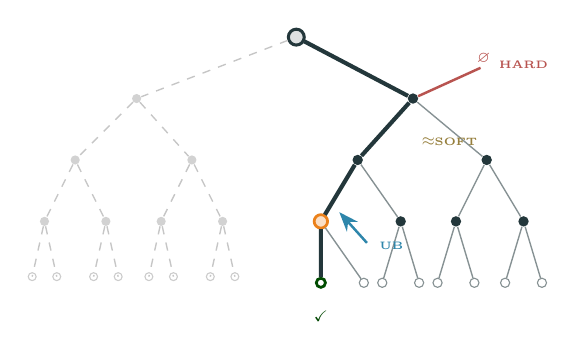
\begin{tikzpicture}[scale=0.78, transform shape,
  exp/.style={circle, fill=navydeep, inner sep=1.7pt},
  fr/.style={circle, draw=mLightBrown, line width=1pt, fill=mLightBrown!25, inner sep=2.2pt},
  leaf/.style={circle, draw=navydeep!55, fill=white, inner sep=1.5pt},
  faint/.style={circle, fill=gray!35, inner sep=1.5pt},
  fleaf/.style={circle, draw=gray!40, fill=white, inner sep=1.3pt},
  pe/.style={navydeep, line width=1.5pt},
  te/.style={navydeep!55, line width=0.5pt},
  fe/.style={gray!45, dashed, line width=0.5pt},
  lbl/.style={font=\tiny\bfseries},
]
  % start node (root)
  \node[circle, draw=navydeep, line width=1.1pt, fill=navydeep!15, inner sep=2.6pt] (R) at (0,4.4) {};
  % ---- pruned LEFT subtree (HARD: whole region cut) ----
  \node[faint] (L)  at (-2.6,3.4) {};
  \node[faint] (L1) at (-3.6,2.4) {}; \node[faint] (L2) at (-1.7,2.4) {};
  \foreach \p/\x in {L1a/-4.1, L1b/-3.1, L2a/-2.2, L2b/-1.2}
    \node[faint] (\p) at (\x,1.4) {};
  \foreach \p/\x in {-4.3,-3.9,-3.3,-2.9,-2.4,-2.0,-1.4,-1.0}
    \node[fleaf] at (\p,0.5) {};
  \draw[fe] (R)--(L); \draw[fe] (L)--(L1) (L)--(L2);
  \draw[fe] (L1)--(L1a) (L1)--(L1b) (L2)--(L2a) (L2)--(L2b);
  \foreach \pp/\xx in {L1a/-4.3,L1a/-3.9,L1b/-3.3,L1b/-2.9,L2a/-2.4,L2a/-2.0,L2b/-1.4,L2b/-1.0}
    \draw[fe] (\pp)--(\xx,0.5);
  % ---- explored RIGHT path ----
  \node[exp] (A) at (1.9,3.4) {};
  \node[exp] (B) at (1.0,2.4) {};   \node[exp] (C) at (3.1,2.4) {};
  \node[fr]  (D) at (0.4,1.4) {};   \node[exp] (E) at (1.7,1.4) {};
  \node[exp] (Cc1) at (2.6,1.4) {}; \node[exp] (Cc2) at (3.7,1.4) {};
  \node[leaf,draw=success!60!black,line width=1pt] (G) at (0.4,0.4) {};
  \node[leaf] (G2) at (1.1,0.4) {};
  \foreach \p/\x in {E1/1.4,E2/2.0,c1a/2.3,c1b/2.9,c2a/3.4,c2b/4.0}
    \node[leaf] (\p) at (\x,0.4) {};
  % path edges (bold)
  \draw[pe] (R)--(A) (A)--(B) (B)--(D) (D)--(G);
  % thin explored edges
  \draw[te] (A)--(C) (B)--(E) (C)--(Cc1) (C)--(Cc2) (D)--(G2);
  \draw[te] (E)--(E1) (E)--(E2) (Cc1)--(c1a) (Cc1)--(c1b) (Cc2)--(c2a) (Cc2)--(c2b);
  % ---- constraint annotations (1 màu / loại) ----
  % HARD (đỏ) cut sibling at level 1
  \draw[cHard, line width=0.9pt] (A) -- (3.0,3.9);
  \node[cHard] at (3.05,4.05) {\scriptsize$\varnothing$};
  \node[lbl, cHard] at (3.7,3.95) {HARD};
  % SOFT (vàng) at level 2
  \node[cSoft!75!black] at (2.15,2.7) {\scriptsize$\approx$};
  \node[lbl, cSoft!75!black] at (2.6,2.7) {SOFT};
  % UPPER (xanh thép) bound arrow near D
  \draw[cUpper, line width=0.9pt, -{Stealth}] (1.15,1.05) -- (0.7,1.55);
  \node[lbl, cUpper] at (1.55,1.0) {UB};
  % feasible leaf check
  \node[success!55!black, font=\scriptsize\bfseries] at (0.4,-0.15) {\checkmark};
\end{tikzpicture}

\vspace{0.3em}
{\centering\footnotesize\itshape\color{gray} HARD / SOFT / UPPER \emph{học từ build} tỉa cây $\to$ 1 path khả thi.\par}
\end{columns}
\end{frame}

\begin{frame}{CGAR: Session-scoped Learning}
\vspace{0.4em}
{\centering\footnotesize\color{mDarkTeal}\textbf{Session = 1 repository = nhiều snippet:} ràng buộc học được \emph{chia sẻ} giữa các snippet trong cùng session.\par}

\vspace{0.3em}
\begin{figure}
    \centering
    \href{https://chatgpt.com/share/6a2a3c8b-93f8-83ec-9452-052ef1ef7e87}{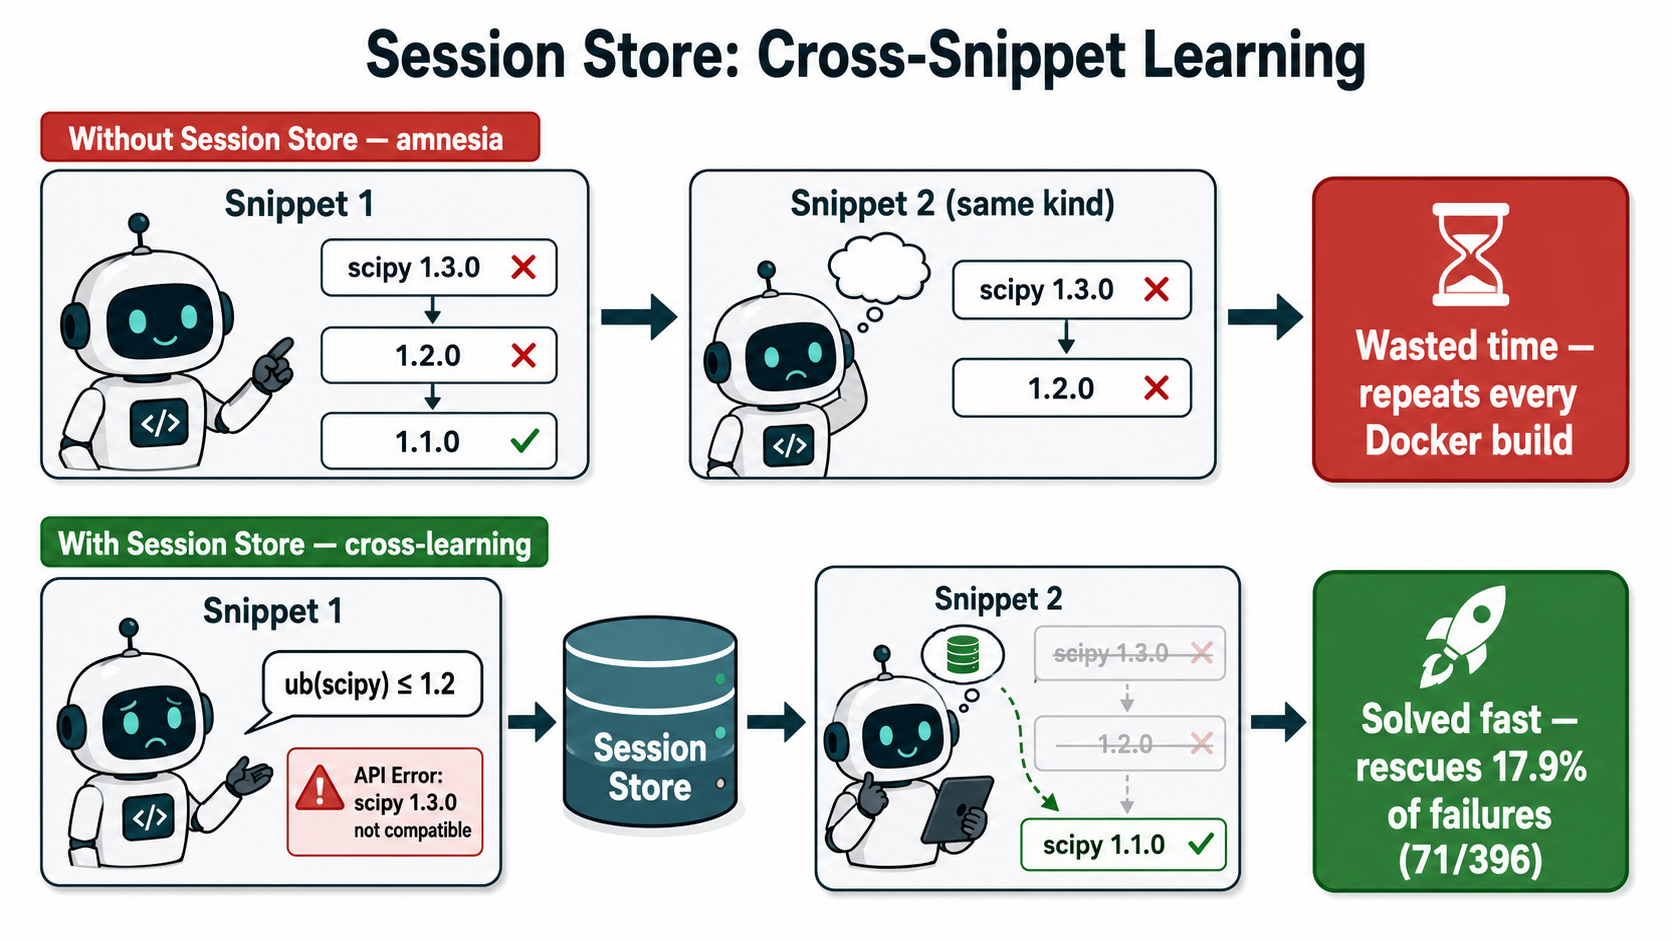
\includegraphics[width=0.82\textwidth]{session-learning.png}}
    \caption{Cơ chế học chéo: Session Store giúp ``cứu'' 17.9\% MEMRES-failures (71/396)}
\end{figure}
\vspace{-0.4em}
{\centering\tiny\color{gray}Minh họa AI, \href{https://chatgpt.com/share/6a2a3c8b-93f8-83ec-9452-052ef1ef7e87}{\textcolor{mLightBrown}{ChatGPT prompt}}\par}
\end{frame}

% ---- Slide Failure Cases (tạm ẩn) ----
% \begin{frame}{Failure Cases}
% \scriptsize
% \begin{tabular}{p{3.2cm} p{4.2cm} p{4cm}}
%   \toprule
%   \textbf{Cách thất bại} & \textbf{Why?} & \textbf{Cách khắc phục} \\
%   \midrule
%   \rowcolor{alert!8}
%   Hardcode bảng API-removal & Rất dễ gãy; sập mỗi khi có API mới bị xóa & Dùng Error Analyzer Agent (LLM) \\
%   \rowcolor{alert!8}
%   Reset store sau mỗi snippet & Lãng phí khả năng học chéo & Session-scoped store (ablation: bỏ store $\Rightarrow -21\%$ rescue) \\
%   \rowcolor{alert!8}
%   Chỉ dùng ràng buộc HARD & Vô tình cấm do lỗi ngẫu nhiên & Thêm mức SOFT (đếm $\ge 2$) \\
%   \rowcolor{alert!8}
%   Không lọc wheel & Build source tốn 3 phút; kẹt ở \textbf{10\%} & \texttt{wheel\_filter()} (ablation: bỏ $\Rightarrow -44\%$ rescue) \\
%   DFS Tham lam (không giới hạn) & Bị kẹt ở không gian rộng $>$ 1000 ứng viên & Giới hạn 50 lần thử + Python pivot \\
%   \bottomrule
% \end{tabular}
%
% \vspace{0.5em}
% \begin{block}{Lesson}
% \scriptsize
% Each failure mode taught us a structural principle: \emph{learn from errors, don't hardcode them}.
% \end{block}
% \end{frame}

% ============================================================
\section{Kết quả}
% ============================================================

% ─── R1. Comprehensive Comparison ──────────────────────────
\begin{frame}{Comprehensive Comparison}
\vspace{1.2em}
\scriptsize
\setlength{\tabcolsep}{4pt}
\renewcommand{\arraystretch}{1.18}
\centering
\begin{tabular}{@{}c l l l r r r c@{}}
  \toprule
  \textbf{\#} & \textbf{Method} & \textbf{Venue} & \textbf{Approach} & \textbf{HG2.9K} & \textbf{GitCham.} & \textbf{Time} & \textbf{Open} \\
  \midrule
  1 & PyEGo                & ICSE'22  & KG + Z3 SMT         & 45.0\%           & --     & 5.8s    & -- \\
  2 & ReadPyE              & TSE'24   & KG + README         & 47.2\%           & --     & 106.9s  & -- \\
  \midrule
  \rowcolor{cInferL}
  3 & GPT-4o               & 2024     & closed LLM          & --               & 49.1\% & --      & \alert{\ding{55}} \\
  \rowcolor{cInferL}
  4 & Gemini 2.5 Pro       & 2025     & closed LLM          & --               & 50.0\% & --      & \alert{\ding{55}} \\
  \rowcolor{cInferL}
  5 & o1                   & 2024     & closed (best)       & --               & 51.2\% & --      & \alert{\ding{55}} \\
  \rowcolor{cInferL}
  6 & GPT-4.1 + RAG        & 2025     & closed LLM + RAG    & --               & 58.5\% & --      & \alert{\ding{55}} \\
  \midrule
  7 & PLLM                 & arXiv'25 & RAG + LLM iter.     & 44.8\%           & 65.5\% & 369.6s  & \textcolor{success}{\ding{51}} \\
  8 & SMT-LLM              & FSE'26   & Z3 SMT + LLM imput. & 83.6\%           & --     & 23.9s\,{\tiny(med)}$^{\dagger}$ & \textcolor{success}{\ding{51}} \\
  9 & \textbf{MEMRES}      & \textbf{FSE'26} & Memory + Cascade & 86.3\% & 81.7\% & 335.3s & \textcolor{success}{\ding{51}} \\
  \rowcolor{accent!18}
  10& \textbf{CGAR}        & \textbf{(ours)} & \textbf{Multi-Agent + CA} & \textcolor{success!50!black}{\textbf{87.1\%}} & \textcolor{success!50!black}{\textbf{83.2\%}} & \textbf{22.3s} & \textcolor{success}{\ding{51}} \\
  \bottomrule
\end{tabular}

\vspace{0.5em}
\tiny PLLM 44.8\% = reproduction single-run (paper headline 54.8\% là 10-run union). \textbf{Time} = avg tất cả snippet (pass+fail) trên HG2.9K. $^{\dagger}$SMT-LLM 23.9s là \emph{median} (paper không báo avg/snippet). SMT-LLM cũng dùng Gemma-2 9B + Docker, đồng venue FSE'26 với MEMRES.\\
\textcolor{mDarkTeal}{\textbf{Fairness}: budget = \textbf{$\le$10 build $\times$ 180s/build $\approx$1800s/snippet, giống nhau mọi tool}. CGAR chỉ cần $\le$5 build để về đích trong cùng trần $\Rightarrow$ time thấp là do \emph{hội tụ nhanh}, không phải budget khác. Speed headline so trên \textbf{GitChameleon} (mọi tool cùng cấu hình).}
\end{frame}

% ─── R2. HG2.9K — In-Distribution Detailed ──────────────────
\begin{frame}{HG2.9K: Error Breakdown}
\vspace{0.6em}
\begin{columns}[c,onlytextwidth]
\column{0.54\textwidth}
\centering
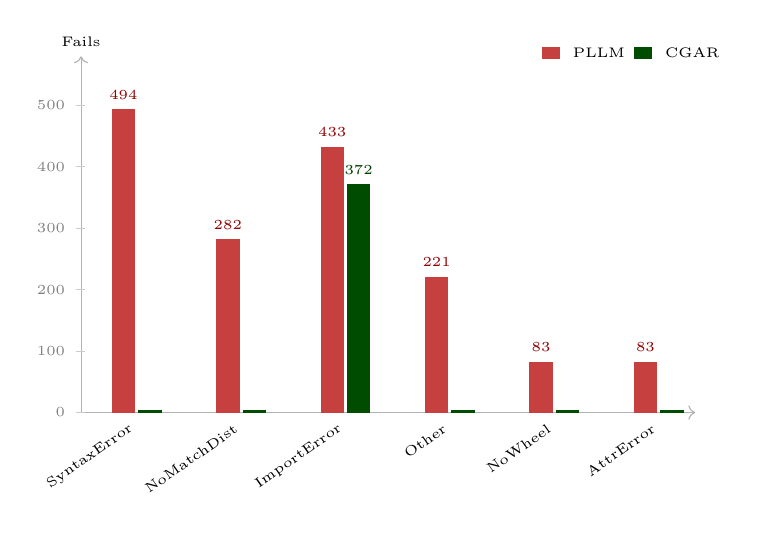
\begin{tikzpicture}[scale=0.78]
  \def\xmax{10.0}\def\ymax{5.5}
  \draw[->, gray!60] (0, 0) -- (\xmax, 0);
  \draw[->, gray!60] (0, 0) -- (0, \ymax+0.3) node[above, font=\tiny, black]{Fails};
  \foreach \y/\v in {0/0, 1/100, 2/200, 3/300, 4/400, 5/500} {
    \draw[gray!40] (-0.08, \y) -- (0.06, \y);
    \node[font=\tiny, gray, anchor=east] at (-0.1, \y) {\v};
  }
  \def\bw{0.38}
  % 1. SyntaxError 494 -> 0
  \fill[alert!75]         (0.5, 0)            rectangle ++(\bw, 4.94);
  \fill[success!60!black] (0.5+\bw+0.05, 0)   rectangle ++(\bw, 0.04);
  \node[font=\tiny, rotate=35, anchor=east] at (0.95, -0.15) {SyntaxError};
  \node[font=\tiny, anchor=south, color=alert!80!black] at (0.5+\bw/2, 4.94) {494};
  % 2. NoMatchDist 282 -> 0
  \fill[alert!75]         (2.2, 0)            rectangle ++(\bw, 2.82);
  \fill[success!60!black] (2.2+\bw+0.05, 0)   rectangle ++(\bw, 0.04);
  \node[font=\tiny, rotate=35, anchor=east] at (2.65, -0.15) {NoMatchDist};
  \node[font=\tiny, anchor=south, color=alert!80!black] at (2.2+\bw/2, 2.82) {282};
  % 3. ImportError 433 -> 372
  \fill[alert!75]         (3.9, 0)            rectangle ++(\bw, 4.33);
  \fill[success!60!black] (3.9+\bw+0.05, 0)   rectangle ++(\bw, 3.72);
  \node[font=\tiny, rotate=35, anchor=east] at (4.35, -0.15) {ImportError};
  \node[font=\tiny, anchor=south, color=alert!80!black] at (3.9+\bw/2, 4.33) {433};
  \node[font=\tiny, anchor=south, color=success!50!black] at (3.9+\bw+0.05+\bw/2, 3.72) {372};
  % 4. Other 221 -> 1
  \fill[alert!75]         (5.6, 0)            rectangle ++(\bw, 2.21);
  \fill[success!60!black] (5.6+\bw+0.05, 0)   rectangle ++(\bw, 0.04);
  \node[font=\tiny, rotate=35, anchor=east] at (6.05, -0.15) {Other};
  \node[font=\tiny, anchor=south, color=alert!80!black] at (5.6+\bw/2, 2.21) {221};
  % 5. NoWheel 83 -> 0
  \fill[alert!75]         (7.3, 0)            rectangle ++(\bw, 0.83);
  \fill[success!60!black] (7.3+\bw+0.05, 0)   rectangle ++(\bw, 0.04);
  \node[font=\tiny, rotate=35, anchor=east] at (7.75, -0.15) {NoWheel};
  \node[font=\tiny, anchor=south, color=alert!80!black] at (7.3+\bw/2, 0.83) {83};
  % 6. AttrError 83 -> 0
  \fill[alert!75]         (9.0, 0)            rectangle ++(\bw, 0.83);
  \fill[success!60!black] (9.0+\bw+0.05, 0)   rectangle ++(\bw, 0.04);
  \node[font=\tiny, rotate=35, anchor=east] at (9.45, -0.15) {AttrError};
  \node[font=\tiny, anchor=south, color=alert!80!black] at (9.0+\bw/2, 0.83) {83};
  % Legend (right side)
  \fill[alert!75]         (7.5, 5.75) rectangle ++(0.3, 0.2);
  \node[font=\tiny, anchor=west] at (7.85, 5.85) {PLLM};
  \fill[success!60!black] (9.0, 5.75) rectangle ++(0.3, 0.2);
  \node[font=\tiny, anchor=west] at (9.35, 5.85) {CGAR};
\end{tikzpicture}

\vspace{0.4em}
\scriptsize CGAR triệt tiêu \textbf{4 nhóm lỗi}; gần như chỉ còn ImportError (99.7\% phần còn lại).\\
Total fails: PLLM \textbf{1596} $\to$ CGAR \textbf{373} \quad\textcolor{success!50!black}{$\Delta\,-76.6\%$}

\hspace{0.04\textwidth}
\column{0.42\textwidth}
\scriptsize
\centering
\textbf{Rescue rate theo PLLM error type}
\vspace{0.4em}

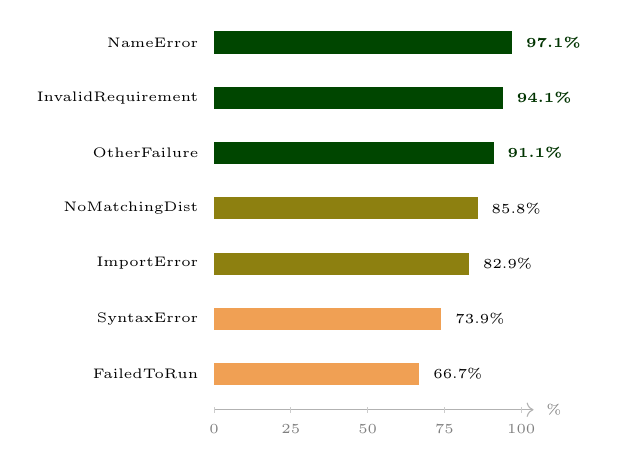
\begin{tikzpicture}[scale=0.78]
  % Horizontal bars: 7 PLLM error types vs CGAR rescue rate (%)
  % Y top to bottom; sorted descending
  \def\xmax{5.2}
  \def\bh{0.36}
  % Scale: 1 unit = 20% -> 100% = 5
  % positions: y = 6.3, 5.4, 4.5, 3.6, 2.7, 1.8, 0.9
  % NameError 97.1
  \fill[success!55!black] (0, 6.3) rectangle ++(4.855, \bh);
  \node[font=\tiny, anchor=east] at (-0.1, 6.48) {NameError};
  \node[font=\tiny, anchor=west, color=success!40!black] at (4.92, 6.48) {\textbf{97.1\%}};
  % InvalidRequirement 94.1
  \fill[success!55!black] (0, 5.4) rectangle ++(4.705, \bh);
  \node[font=\tiny, anchor=east] at (-0.1, 5.58) {InvalidRequirement};
  \node[font=\tiny, anchor=west, color=success!40!black] at (4.77, 5.58) {\textbf{94.1\%}};
  % OtherFailure 91.1
  \fill[success!55!black] (0, 4.5) rectangle ++(4.555, \bh);
  \node[font=\tiny, anchor=east] at (-0.1, 4.68) {OtherFailure};
  \node[font=\tiny, anchor=west, color=success!40!black] at (4.62, 4.68) {\textbf{91.1\%}};
  % NoMatchingDist 85.8
  \fill[success!40!mLightBrown] (0, 3.6) rectangle ++(4.29, \bh);
  \node[font=\tiny, anchor=east] at (-0.1, 3.78) {NoMatchingDist};
  \node[font=\tiny, anchor=west] at (4.36, 3.78) {85.8\%};
  % ImportError 82.9
  \fill[success!40!mLightBrown] (0, 2.7) rectangle ++(4.145, \bh);
  \node[font=\tiny, anchor=east] at (-0.1, 2.88) {ImportError};
  \node[font=\tiny, anchor=west] at (4.22, 2.88) {82.9\%};
  % SyntaxError 73.9
  \fill[mLightBrown!75] (0, 1.8) rectangle ++(3.695, \bh);
  \node[font=\tiny, anchor=east] at (-0.1, 1.98) {SyntaxError};
  \node[font=\tiny, anchor=west] at (3.77, 1.98) {73.9\%};
  % FailedToRun 66.7
  \fill[mLightBrown!75] (0, 0.9) rectangle ++(3.335, \bh);
  \node[font=\tiny, anchor=east] at (-0.1, 1.08) {FailedToRun};
  \node[font=\tiny, anchor=west] at (3.41, 1.08) {66.7\%};
  % X axis
  \draw[->, gray!60] (0, 0.5) -- (\xmax, 0.5);
  \foreach \x/\v in {0/0, 1.25/25, 2.5/50, 3.75/75, 5/100} {
    \draw[gray!40] (\x, 0.45) -- (\x, 0.55);
    \node[font=\tiny, gray, anchor=north] at (\x, 0.42) {\v};
  }
  \node[font=\tiny, gray, anchor=west] at (\xmax+0.05, 0.5) {\%};
\end{tikzpicture}

\vspace{0.3em}
\tiny CGAR rescue \textbf{80.6\%} (1286/1596) toàn bộ PLLM failures trên HG2.9K.
\end{columns}
\end{frame}

% ─── R3. GitChameleon — Out-of-Distribution ────────────────
\begin{frame}{GitChameleon: Open vs Closed}
\vspace{0.4em}
\begin{columns}[T,onlytextwidth]
\column{0.52\textwidth}
\centering
\scriptsize
\textbf{Full leaderboard}
\vspace{0.3em}

\setlength{\tabcolsep}{6pt}
\renewcommand{\arraystretch}{1.22}
\begin{tabular}{@{}l l r c@{}}
  \toprule
  \textbf{Method} & \textbf{Type} & \textbf{Pass} & \textbf{Open} \\
  \midrule
  \rowcolor{cInferL} GPT-4o            & closed gen    & 49.1\% & \alert{\ding{55}} \\
  \rowcolor{cInferL} Gemini 2.5 Pro    & closed gen    & 50.0\% & \alert{\ding{55}} \\
  \rowcolor{cInferL} o1                & closed (best) & 51.2\% & \alert{\ding{55}} \\
  \rowcolor{cInferL} GPT-4.1 + RAG     & closed + RAG  & 58.5\% & \alert{\ding{55}} \\
  \midrule
  PLLM (Gemma-2 9B)   & open + RAG      & 65.5\% & \textcolor{success}{\ding{51}} \\
  \textbf{MEMRES}     & open + Memory   & 81.7\% & \textcolor{success}{\ding{51}} \\
  \rowcolor{accent!22}
  \textbf{CGAR}       & open + Agent+CA & \textcolor{success!50!black}{\textbf{83.2\%}} & \textcolor{success}{\ding{51}} \\
  \bottomrule
\end{tabular}

\hspace{0.06\textwidth}
\column{0.42\textwidth}
\centering
\scriptsize
\textbf{Cross-benchmark generalization}
\vspace{0.3em}

\setlength{\tabcolsep}{6pt}
\renewcommand{\arraystretch}{1.22}
\begin{tabular}{@{}l r r r@{}}
  \toprule
  \textbf{Tool} & \textbf{HG2.9K} & \textbf{GitCham.} & \textbf{Gap} \\
  \midrule
  PLLM            & 44.8\% & 65.5\% & \alert{$-$20.7pp} \\
  MEMRES          & 86.3\% & 81.7\% & $-$4.6pp \\
  \rowcolor{accent!22}
  \textbf{CGAR}   & \textcolor{success!50!black}{\textbf{87.1\%}} & \textcolor{success!50!black}{\textbf{83.2\%}} & \textcolor{success!50!black}{\textbf{$-$3.9pp}} \\
  \bottomrule
\end{tabular}

\vspace{0.6em}
\tiny \textit{(closed baselines từ arXiv 2507.12367)}
\end{columns}

\vspace{0.9em}
\centering\footnotesize\color{mDarkTeal}
CGAR (open 9B, $<$10\,GB VRAM) vượt o1 (closed, $>$200B params) \textbf{+32.0pp} trên GitChameleon: \emph{system design $>$ raw model scale}.
\end{frame}

% ─── R4. Speed & Efficiency ───────────────────────────────
\begin{frame}{Speed \& Ablation}
\vspace{1.2em}
\begin{columns}[c,onlytextwidth]
\column{0.50\textwidth}
\centering
\scriptsize
\textbf{Duration (GitChameleon)}\\
{\tiny\color{gray}cùng budget $K_{\text{build}}=5$ vòng Docker build cho cả 3 tool}
\vspace{0.4em}

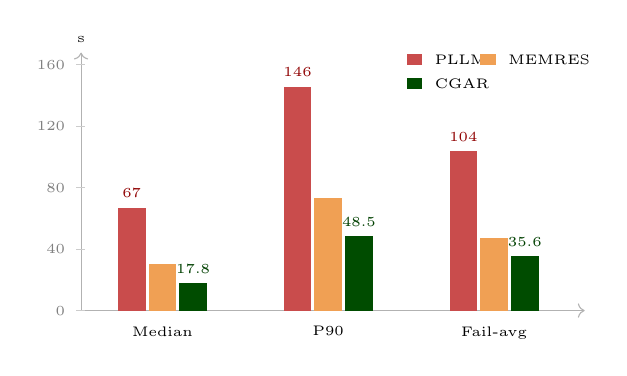
\begin{tikzpicture}[scale=0.78]
  \draw[->, gray!60] (0, 0) -- (8.2, 0);
  \draw[->, gray!60] (0, 0) -- (0, 4.2) node[above, font=\tiny, black]{s};
  \foreach \y/\v in {0/0, 1/40, 2/80, 3/120, 4/160} {
    \draw[gray!40] (-0.08, \y) -- (0.06, \y);
    \node[font=\tiny, gray, anchor=east] at (-0.1, \y) {\v};
  }
  \def\bw{0.45}
  \fill[alert!70]         (0.6, 0) rectangle ++(\bw, 1.675);
  \fill[mLightBrown!75]   (1.1, 0) rectangle ++(\bw, 0.7525);
  \fill[success!60!black] (1.6, 0) rectangle ++(\bw, 0.445);
  \node[font=\tiny, anchor=north] at (1.325, -0.1) {Median};
  \fill[alert!70]         (3.3, 0) rectangle ++(\bw, 3.6475);
  \fill[mLightBrown!75]   (3.8, 0) rectangle ++(\bw, 1.825);
  \fill[success!60!black] (4.3, 0) rectangle ++(\bw, 1.2125);
  \node[font=\tiny, anchor=north] at (4.025, -0.1) {P90};
  \fill[alert!70]         (6.0, 0) rectangle ++(\bw, 2.595);
  \fill[mLightBrown!75]   (6.5, 0) rectangle ++(\bw, 1.18);
  \fill[success!60!black] (7.0, 0) rectangle ++(\bw, 0.89);
  \node[font=\tiny, anchor=north] at (6.725, -0.1) {Fail-avg};
  \node[font=\tiny, anchor=south, color=alert!80!black] at (0.825, 1.675) {67};
  \node[font=\tiny, anchor=south, color=success!50!black] at (1.825, 0.445) {17.8};
  \node[font=\tiny, anchor=south, color=alert!80!black] at (3.525, 3.6475) {146};
  \node[font=\tiny, anchor=south, color=success!50!black] at (4.525, 1.2125) {48.5};
  \node[font=\tiny, anchor=south, color=alert!80!black] at (6.225, 2.595) {104};
  \node[font=\tiny, anchor=south, color=success!50!black] at (7.225, 0.89) {35.6};
  \fill[alert!70] (5.3, 4.0) rectangle ++(0.25, 0.18);
  \node[font=\tiny, anchor=west] at (5.6, 4.09) {PLLM};
  \fill[mLightBrown!75] (6.5, 4.0) rectangle ++(0.25, 0.18);
  \node[font=\tiny, anchor=west] at (6.8, 4.09) {MEMRES};
  \fill[success!60!black] (5.3, 3.6) rectangle ++(0.25, 0.18);
  \node[font=\tiny, anchor=west] at (5.6, 3.69) {CGAR};
\end{tikzpicture}

\hspace{0.04\textwidth}
\column{0.46\textwidth}
\centering
\scriptsize
\textbf{Ablation: CGAR rescue (n=396)}
\vspace{0.4em}

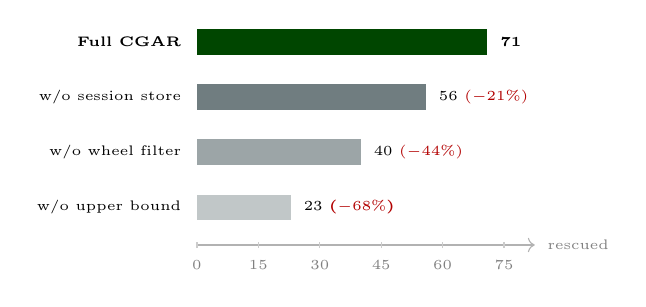
\begin{tikzpicture}[scale=0.78]
  \def\xmax{5.5}
  \def\bh{0.42}
  \fill[success!55!black] (0, 3.3) rectangle ++(4.73, \bh);
  \node[font=\tiny, anchor=east] at (-0.1, 3.51) {\textbf{Full CGAR}};
  \node[font=\tiny, anchor=west] at (4.78, 3.51) {\textbf{71}};
  \fill[mDarkTeal!65] (0, 2.4) rectangle ++(3.73, \bh);
  \node[font=\tiny, anchor=east] at (-0.1, 2.61) {w/o session store};
  \node[font=\tiny, anchor=west] at (3.78, 2.61) {56 \textcolor{alert}{($-21\%$)}};
  \fill[mDarkTeal!45] (0, 1.5) rectangle ++(2.67, \bh);
  \node[font=\tiny, anchor=east] at (-0.1, 1.71) {w/o wheel filter};
  \node[font=\tiny, anchor=west] at (2.72, 1.71) {40 \textcolor{alert}{($-44\%$)}};
  \fill[mDarkTeal!28] (0, 0.6) rectangle ++(1.53, \bh);
  \node[font=\tiny, anchor=east] at (-0.1, 0.81) {w/o upper bound};
  \node[font=\tiny, anchor=west] at (1.58, 0.81) {23 \textcolor{alert}{\textbf{($-68\%$)}}};
  \draw[->, gray!60] (0, 0.2) -- (\xmax, 0.2);
  \foreach \x/\v in {0/0, 1/15, 2/30, 3/45, 4/60, 5/75} {
    \draw[gray!40] (\x, 0.15) -- (\x, 0.25);
    \node[font=\tiny, gray, anchor=north] at (\x, 0.1) {\v};
  }
  \node[font=\tiny, gray, anchor=west] at (\xmax+0.05, 0.2) {rescued};
\end{tikzpicture}
\end{columns}

\vspace{1.0em}
\centering\footnotesize\color{mDarkTeal}
\emph{``The best build is the one you never run.''}\\[0.2em]
\scriptsize\color{black}
\textbf{Multi-agent nhưng nhanh nhất}: solver tỉa không gian $\Rightarrow$ ít Docker build; fail chỉ chậm hơn pass \textbf{1.31$\times$} (PLLM 2.20$\times$).
\end{frame}

% ============================================================
\section{Hạn chế \& Hướng phát triển}
% ============================================================

% --- Limitations slide ---
\begin{frame}{Hạn chế: Hard Floor \& Architectural Limits}
\vspace{0.3em}
\begin{columns}[T,onlytextwidth]
\column{0.50\textwidth}
\centering
\scriptsize
\textbf{Hard Floor: 310 snippets (10.7\%)}\\
{\tiny\color{gray}cả PLLM và CGAR đều fail}
\vspace{0.4em}

\setlength{\tabcolsep}{5pt}
\renewcommand{\arraystretch}{1.22}
\begin{tabular}{@{}l r@{}}
  \toprule
  \textbf{Root cause} & \textbf{Share} \\
  \midrule
  Python 2 syntax (no Py2 wheel)        & 41.6\% \\
  ImportError system/private pkg        & 25.8\% \\
  NoMatchingDist (pkg absent)           & 13.3\% \\
  CouldNotBuildWheels (glibc/native)    & 8.1\%  \\
  API removed (no compat older)         & 4.0\%  \\
  Other                                 & 7.2\%  \\
  \bottomrule
\end{tabular}

\vspace{0.5em}
\tiny\color{alert!85!black}
\textit{Irreducible under current constraints} (Docker, PyPI public, no source patching, $\le$10 retries), không phải lỗi tool.

\hspace{0.04\textwidth}
\column{0.46\textwidth}
\scriptsize
\textbf{\color{navydeep}Hạn chế kiến trúc}
\vspace{0.4em}

\begin{itemize}\setlength{\itemsep}{0.5em}
  \item \textcolor{alert!80!black}{\textbf{Phụ thuộc PyPI live:}}
        nếu PyPI down hoặc rate-limit, solver không thể query metadata $\to$ fallback to MEMRES cascade.
  \item \textcolor{alert!80!black}{\textbf{Single ecosystem:}}
        chỉ Python, chưa generalize sang JS / Rust / Go.
  \item \textcolor{alert!80!black}{\textbf{LLM Analyzer brittle với log lạ:}}
        Gemma-2 9B có thể parse sai constraint khi error log có format ngoài pretrain.
  \item \textcolor{alert!80!black}{\textbf{Single-worker session store:}}
        chưa hỗ trợ multi-user federated learning.
\end{itemize}
\end{columns}
\end{frame}

% --- Future Work slide ---
\begin{frame}{Hướng phát triển}
\vspace{0.3em}
\centering
\begin{tikzpicture}[font=\scriptsize,
  fwcard/.style={draw=mLightBrown!45, fill=mLightBrown!5, rounded corners=6pt, line width=1pt,
                 text width=5.3cm, minimum height=1.95cm, align=left, inner sep=10pt, anchor=center},
  wm/.style={font=\Huge\bfseries, text=mLightBrown!25},
]
  \def\xl{-3.2}\def\xr{3.2}\def\yt{1.55}\def\yb{-0.75}
  \node[fwcard] (c1) at (\xl,\yt) {\textbf{\normalsize\color{navydeep}Mở rộng đa ngôn ngữ}\\[3pt]{\tiny Áp dụng CGAR cho \textbf{npm}, \textbf{cargo}, \textbf{go.mod}; bộ giải không phụ thuộc ecosystem, chỉ cần adapter cho từng registry.}};
  \node[fwcard] (c2) at (\xr,\yt) {\textbf{\normalsize\color{navydeep}Chia sẻ constraint}\\[3pt]{\tiny Federated, bảo toàn riêng tư: snippet user A fix giúp user B tránh lỗi tương tự, tận dụng quy mô cộng đồng.}};
  \node[fwcard] (c3) at (\xl,\yb) {\textbf{\normalsize\color{navydeep}Tinh chỉnh LLM đọc lỗi}\\[3pt]{\tiny Fine-tune Gemma-2 trên dữ liệu \textbf{đọc log} chuyên dụng để phân loại đúng lỗi, sinh constraint chính xác hơn.}};
  \node[fwcard] (c4) at (\xr,\yb) {\textbf{\normalsize\color{navydeep}Mở rộng đa mô hình}\\[3pt]{\tiny Chạy CGAR trên nhiều LLM backbone (Qwen3, Phi, Llama\dots) và các \textbf{model nhỏ/rẻ} hơn, chứng minh phương pháp không phụ thuộc một model cụ thể.}};
  \node[wm, anchor=north east] at ([xshift=-5pt,yshift=-3pt]c1.north east) {1};
  \node[wm, anchor=north east] at ([xshift=-5pt,yshift=-3pt]c2.north east) {2};
  \node[wm, anchor=north east] at ([xshift=-5pt,yshift=-3pt]c3.north east) {3};
  \node[wm, anchor=north east] at ([xshift=-5pt,yshift=-3pt]c4.north east) {4};
\end{tikzpicture}

\vspace{0.5em}
{\centering\footnotesize\color{mDarkTeal}\textbf{Mục tiêu dài hạn:} từ bộ giải cho Python trở thành \textbf{``environment archaeologist''} đa năng cho mọi ecosystem.\par}
\end{frame}

\begin{frame}{Tài liệu tham khảo}
\vspace{0.3em}
\scriptsize
\setbeamertemplate{enumerate items}{\color{mDarkTeal}\bfseries[\insertenumlabel]}
\begin{enumerate}\setlength{\itemsep}{0.22em}\setlength{\parsep}{0pt}
  \item E. Horton and C. Parnin, ``Gistable: Evaluating the executability of Python code snippets on GitHub,'' in \textit{Proc. ICSME}, 2018. {\color{gray}(dataset HG2.9K; arXiv:1808.04919)}
  \item H. Ye, W. Chen, W. Dou, G. Wu, and J. Wei, ``Knowledge-based environment dependency inference for Python programs (PyEGo),'' in \textit{Proc. ICSE}, 2022.
  \item ``Revisiting knowledge-based inference of Python runtime environments (ReadPyE),'' \textit{IEEE Trans. Softw. Eng.}, vol. 50, 2024.
  \item S. Mukherjee, A. Almanza, and C. Rubio-González, ``Fixing dependency errors for Python build reproducibility (PyDFix),'' in \textit{Proc. ISSTA}, 2021.
  \item A. Bartlett, C. C. S. Liem, and A. Panichella, ``Raiders of the lost dependency: Fixing dependency conflicts in Python using LLMs (PLLM),'' \textit{arXiv:2501.16191}, 2025.
  \item ``GitChameleon 2.0: Evaluating AI code generation against Python library version incompatibilities,'' \textit{arXiv:2507.12367}, 2025.
  \item N. Shinn \textit{et al.}, ``Reflexion: Language agents with verbal reinforcement learning,'' in \textit{Proc. NeurIPS}, 2023.
  \item L. de Moura and N. Bjørner, ``Z3: An efficient SMT solver,'' in \textit{Proc. TACAS}, 2008.
  \item ``SMT-LLM: Z3 SMT $+$ LLM imputation for dependency resolution,'' FSE-AIWare 2026 competition entry, unpublished (reproduced by our group).
\end{enumerate}
\end{frame}

% ─── Video demo: clickable thumbnail -> video link ───
\def\videourl{https://www.facebook.com/share/v/17m6jVkP5F/}
\begin{frame}{Video trình bày (\texorpdfstring{$\sim$}{~}6 phút)}
\centering
\vspace{0.2em}
\href{\videourl}{%
  \IfFileExists{figures/video-demo.png}%
    {
\includegraphics[height=0.62\textheight]{video-demo.png}}%
    {\fcolorbox{navydeep!40}{softgray}{\parbox[c][0.55\textheight][c]{0.78\textwidth}{\centering
       {\Huge\color{navydeep!60}$\triangleright$}\\[0.7em]
       {\normalsize\color{gray}\texttt{figures/video-demo.png}}\\[0.4em]
       {\scriptsize\color{gray}(lưu ảnh capture vào đây, slide tự hiện)}}}}%
}

\vspace{0.6em}
{\footnotesize\color{mDarkTeal} Bấm vào ảnh để xem video demo (\href{\videourl}{mở liên kết}).\par}
\end{frame}

\begin{frame}{Thank you!}
\vspace{2em}
\centering
\Large\textbf{\color{mDarkTeal}Cảm ơn đã lắng nghe!}\\[1em]
\large\textit{Questions \& Discussion}

\vspace{2em}
\scriptsize
\begin{columns}[c]
\column{0.18\textwidth}
\centering
\href{https://www.hcmus.edu.vn}{
\includegraphics[height=1.4cm]{hcmus.png}}

\column{0.64\textwidth}
\centering
\textcolor{navydeep}{MEMRES $\to$ CGAR: Agentic Python Dependency Resolution}\\[0.3em]
Trần Chí Nguyên · Đào Sỹ Duy Minh · Huỳnh Trung Kiệt
\vspace{0.3em}

University of Science, VNU-HCM

\column{0.18\textwidth}
\centering
\href{https://conf.researchr.org/home/fse-2026}{
\includegraphics[height=1.1cm]{fse.png}}
\end{columns}
\end{frame}

% ============================================================
% BACKUP SLIDES (for Q&A)
% ============================================================
\appendix

% [HIDDEN] slide MEMRES Stage Details -- bat lai: xoa dong iffalse ngay duoi + dong fi sau end frame
\iffalse
\begin{frame}{Backup: MEMRES Stage Details}
\vspace{0.3em}

\centering
\begin{tikzpicture}[
  every node/.style={font=\tiny},
  stage/.style={draw=navydeep, fill=navydeep!6, rounded corners=4pt,
                minimum width=5.6cm, minimum height=2.0cm, align=left,
                inner sep=6pt, line width=0.8pt, anchor=north west},
  side/.style={draw=mLightBrown, fill=mLightBrown!8, rounded corners=4pt,
               minimum width=5.6cm, minimum height=2.0cm, align=left,
               inner sep=6pt, line width=0.8pt, anchor=north west},
]

% Row 1
\node[stage] at (-5.9, 2.6) {%
  \textbf{\color{navydeep}\scriptsize Stage 1: Intra-Session Memory}\\[3pt]
  $\blacktriangleright$ Cache solution từ snippet đã fixed trong batch\\
  $\blacktriangleright$ Match qua \textbf{Jaccard $\ge$ 0.5} trên import sets\\
  $\blacktriangleright$ Reapply qua \textbf{1 pip install} duy nhất\\
  $\blacktriangleright$ Reset giữa runs $\to$ no cross-run overfitting%
};

\node[stage] at (-0.1, 2.6) {%
  \textbf{\color{navydeep}\scriptsize Stage 2: Hybrid Evaluation}\\[3pt]
  $\blacktriangleright$ Static regex + \textbf{Semantic Import Analyzer}\\
  $\blacktriangleright$ \textbf{13 usage patterns}: \texttt{(import,call)$\to$pkg}\\
  \;\;\;\;\textcolor{gray}{VD: \texttt{Image.open()}$\to$Pillow}\\
  $\blacktriangleright$ \textbf{11 ecosystems} · 11 code patterns\\
  $\blacktriangleright$ \textbf{Py2 detector}: 13 Py2 + 5 Py3 indicators%
};

% Row 2
\node[stage] at (-5.9, 0.4) {%
  \textbf{\color{navydeep}\scriptsize Stage 3: Confidence Cascade (6 levels)}\\[3pt]
  $\blacktriangleright$ L1 Session · L2 Compat Map (40+pkg$\times$8Py)\\
  $\blacktriangleright$ L3 Templates (23 sets) · L5 Heuristics (45+)\\
  $\blacktriangleright$ L4 Co-occurrence (50K req.txt, pre-2020)\\
  $\blacktriangleright$ L6 \textbf{LLM} (last resort) ·  conf $\ge$ 7 / 3%
};

\node[stage] at (-0.1, 0.4) {%
  \textbf{\color{navydeep}\scriptsize Stage 4: Build Loop + Reflexion}\\[3pt]
  $\blacktriangleright$ Docker build, $\le$\textbf{10 retries}, 180s/build\\
  $\blacktriangleright$ \textbf{Sys-dep inject}: 35+ pip$\to$apt mappings\\
  $\blacktriangleright$ \textbf{Version fallback}: numpy 1.16$\to$1.15$\to$1.14\\
  $\blacktriangleright$ \textbf{Reflexion} (NeurIPS'23) verbal RL retry%
};

% Row 3 — side memories (orange)
\node[side] at (-5.9, -1.8) {%
  \textbf{\color{mLightBrown}\scriptsize Self-Evolving Memory} \textit{\tiny(Mobile-Agent-E)}\\[3pt]
  $\blacktriangleright$ \textbf{Tips} = NL guidelines (cross-snippet)\\
  $\blacktriangleright$ \textbf{Shortcuts} = validated solutions (Jaccard$\ge$0.5)\\
  $\blacktriangleright$ Sandboxed Docker validate trước khi commit\\
  $\blacktriangleright$ Anti-pattern: per-package failure stats%
};

\node[side] at (-0.1, -1.8) {%
  \textbf{\color{mLightBrown}\scriptsize Error Pattern KB}\\[3pt]
  $\blacktriangleright$ \textbf{200+} import$\to$pip mappings (15 domains)\\
  $\blacktriangleright$ \textbf{35} name corrections · \textbf{8} regex rules\\
  $\blacktriangleright$ Version constraints cho 14 packages\\
  $\blacktriangleright$ Self-learning at runtime, no HG2.9K leakage%
};
\end{tikzpicture}

\vspace{0.4em}
\centering\scriptsize\color{success!55!black}
\textbf{Hiệu quả:} self-learning at runtime, no HG2.9K leakage
\end{frame}
\fi
% [end HIDDEN: MEMRES Stage Details]

% [HIDDEN] slide GitChameleon Re-framing -- bat lai: xoa dong iffalse ngay duoi + dong fi sau end frame
\iffalse
\begin{frame}[fragile]{Backup: GitChameleon Re-framing}
\vspace{0.3em}
\scriptsize
\textit{GitChameleon gốc là \textbf{code-generation benchmark} cho LLM ``viết code đúng version''. Mình \textbf{re-frame} thành dependency resolution test.}

\vspace{0.5em}
\begin{columns}[T,onlytextwidth]
\column{0.48\textwidth}
\centering
\textbf{Gốc: 1 JSON / example}
\vspace{0.3em}

\begin{lstlisting}[language=, basicstyle=\tiny\ttfamily, keywordstyle=]
{
  "example_id": 0,
  "library": "torch",
  "version": "1.9",
  "python_version": "3.6",
  "starting_code": "import torch\ndef ...",
  "solution": "    import numpy ...\n    ...",
  "test": "assert torch.allclose(...)",
  "extra_dependencies": ["numpy","scipy"]
}
\end{lstlisting}

\tiny\color{gray}
3 phần tách biệt: starting / solution / test\\
LLM thấy starting + version $\to$ generate body $\to$ chấm bằng test.

\hspace{0.04\textwidth}
\column{0.48\textwidth}
\centering
\textbf{Sau convert: 1 snippet runnable}
\vspace{0.3em}

\begin{lstlisting}[basicstyle=\tiny\ttfamily]
import torch
def log_ndtr(input_tensor):
    import numpy as np
    from scipy.stats import norm
    output = torch.from_numpy(
        norm.logcdf(input_tensor.numpy()))
    return output

# --- test ---
input_tensor = torch.linspace(-10,10,20)
assert torch.allclose(log_ndtr(...), ...)
\end{lstlisting}

\tiny\color{gray}
Concat starting+solution+test thành 1 file.\\
Version \textbf{giấu} $\to$ lưu riêng \texttt{ground\_truth.csv}.
\end{columns}

\vspace{0.5em}
\centering\footnotesize\color{mDarkTeal}
\textbf{Tại sao khó hơn HG2.9K:}\\[0.2em]
\scriptsize\color{black}
Success = \textbf{pass unit test} (semantic correctness), không phải chỉ \texttt{import} chạy được.
Cài \texttt{torch==2.0} thay vì \texttt{1.9} vẫn import OK nhưng \texttt{assert} fail $\to$ tool bắt buộc pick đúng version.
\end{frame}
\fi
% [end HIDDEN: GitChameleon Re-framing]

% ============================================================
% ─── Backup: Filter & Constraint Solver I/O ─────────────────
% ============================================================
\begin{frame}[fragile]{Backup: Filter \& Constraint Solver (I/O)}
\vspace{0.2em}
\scriptsize
\begin{columns}[T,onlytextwidth]
\column{0.49\textwidth}
\textbf{\color{navydeep}Filter: CandidateGraphBuilder}\\[0.2em]
\textit{candidate\_graph\_builder.py}
\begin{lstlisting}[basicstyle=\tiny\ttfamily, language=Python]
Input : packages = ["scipy", "numpy"]
        python_version = "3.7"

# Per package:
#   GET https://pypi.org/pypi/<pkg>/json
#   filter requires_python by SpecifierSet
#   wheel filter (linux/x86_64 only):
#     "-none-any.whl"   | "manylinux"
#     | "linux_x86_64"  | "-cp37-" | "-py3-"
#   sort: wheel-first, newest-first
#   take top 8

Output: {
  "scipy": [
    {v:"1.7.3", requires_python:">=3.7",
     has_wheel:True},
    {v:"1.7.2", ..., has_wheel:True},
    ... up to 8 candidates
  ],
  "numpy": [...]
}
\end{lstlisting}

\column{0.49\textwidth}
\textbf{\color{navydeep}Solver: ConstraintSolver}\\[0.2em]
\textit{constraint\_solver.py:51-123}
\begin{lstlisting}[basicstyle=\tiny\ttfamily, language=Python]
Input : graph (from Filter)
        python_version
        exclude_combo  # last failed pick

# 1. viable = filter graph by store
#    (HARD/SOFT/UpperBound pruning)
# 2. greedy: pick newest viable per pkg
# 3. if combo in exclude or infeasible:
#      _next_assignment(): odometer-style
#      enumeration, skip known-bad combos
#      max_attempts = 50 (safety cap)
#                     ^^^ logic-only,
#                         no Docker calls

Output: {"scipy":"1.7.3","numpy":"1.21.6"}
        or None if exhausted
\end{lstlisting}
\end{columns}

\vspace{0.3em}
\centering\tiny\color{gray}
\textbf{Two Ks:} $K_{\text{solve}}\!=\!50$ logical attempts/solve call (dict-lookup, $\mu$s) ·
$K_{\text{build}}\!\le\!10$ Docker retries/snippet (180s/build, expensive).
\end{frame}

% ============================================================
% ─── Backup: Agent ↔ Agent Communication ────────────────────
% ============================================================
\begin{frame}[fragile]{Backup: Agent Communication (Message I/O)}
\vspace{0.1em}
{\tiny\color{gray}\textit{cgar\_resolver.py · loose-coupled via shared ConstraintStore (no direct calls between agents)}}
\vspace{0.3em}
\scriptsize
\begin{columns}[T,onlytextwidth]
\column{0.50\textwidth}
\textbf{\color{navydeep}1. Planner $\to$ Executor}\\[0.1em]
\textit{assignment dict}
\begin{lstlisting}[basicstyle=\tiny\ttfamily, language=Python]
{"scipy": "1.7.3", "numpy": "1.21.6",
 "matplotlib": "3.5.3"}
\end{lstlisting}

\vspace{0.3em}
\textbf{\color{navydeep}2. Executor $\to$ Analyzer}\\[0.1em]
\textit{build result + error log}
\begin{lstlisting}[basicstyle=\tiny\ttfamily, language=Python]
{"success": False,
 "error_type": "ImportError",
 "error_log": "ImportError: cannot
   import name 'imread' from 'scipy.misc'",
 "assignment": {"scipy":"1.7.3",...}}
\end{lstlisting}

\vspace{0.3em}
\textbf{\color{navydeep}3. Analyzer $\to$ Store (write)}\\[0.1em]
\textit{store.add\_upper\_bound() / inject()}
\begin{lstlisting}[basicstyle=\tiny\ttfamily, language=Python]
add_upper_bound("scipy", "3.7", "1.3")
# scipy >= 1.3 infeasible on py3.7
# (imread removed in scipy 1.3)
\end{lstlisting}

\column{0.50\textwidth}
\textbf{\color{navydeep}4. Store $\to$ Planner (read)}\\[0.1em]
\textit{next round, planner queries store}
\begin{lstlisting}[basicstyle=\tiny\ttfamily, language=Python]
store.get_upper_bound("scipy", "3.7")
# -> "1.3"
store.get_infeasible_versions("scipy","3.7")
# -> {"1.7.3", "1.6.0", ...}
# Planner's solver prunes these
\end{lstlisting}

\vspace{0.3em}
\textbf{\color{navydeep}5. Analyzer $\to$ Critic}\\[0.1em]
\textit{critic.record\_failure() per build}
\begin{lstlisting}[basicstyle=\tiny\ttfamily, language=Python]
{"assignment": {"scipy":"1.7.3",...},
 "python_version": "3.7",
 "error_type": "ImportError"}
\end{lstlisting}

\vspace{0.3em}
\textbf{\color{navydeep}6. Critic $\to$ Orchestrator}\\[0.1em]
\textit{strategic action (fires when stuck)}
\begin{lstlisting}[basicstyle=\tiny\ttfamily, language=Python]
{"action": "switch_python",
 "target": "2.7",
 "reason": "repeated SyntaxError
            -> likely Python 2 code",
 "source": "llm"}
\end{lstlisting}
\end{columns}

\vspace{0.3em}
\centering\tiny\color{gray}
\textbf{Coupling:} agents never call each other directly, coordinator (\texttt{CGARResolver}) drives the loop;
shared \texttt{ConstraintStore} carries cross-snippet knowledge within a session.
\end{frame}

% ============================================================
% ─── Backup: ConstraintStore Data Structures ────────────────
% ============================================================
\begin{frame}[fragile]{Backup: Session Store Data Structures}
\vspace{-0.2em}
{\tiny\color{gray}\textit{constraint\_store.py · failure\_injector.py · shared across all agents in 1 session}}
\vspace{0.1em}
\begin{columns}[T,onlytextwidth]
\column{0.50\textwidth}
{\scriptsize\textbf{\color{navydeep}1. InfeasibleRecord + 3 stores}}
\begin{lstlisting}[basicstyle=\tiny\ttfamily, language=Python]
@dataclass
class InfeasibleRecord:
  package, version, python_version: str
  error_type:      ConstraintType  # HARD|SOFT
  error_signature: str   # normalized log
  confidence:      float # 1.0 HARD, 0.8 SOFT
  count:           int   # ++ on re-observation

_records:       Dict[(pkg,ver,py) ->
                     InfeasibleRecord]
_combo_records: Dict[(FrozenSet,py) -> sig]
_upper_bounds:  Dict[(pkg,py) -> version_str]
\end{lstlisting}

{\scriptsize\textbf{\color{navydeep}2. Regex classifiers}}
\begin{lstlisting}[basicstyle=\tiny\ttfamily, language=Python]
_HARD = ["requires a different Python",
  "No matching distribution found", ...]
_SOFT = ["ImportError","ModuleNotFoundError",
  "cannot import name", ...]
_API_REMOVED_RE =
  r"cannot import name '(\w+)' from '([\w.]+)'"
\end{lstlisting}

\column{0.50\textwidth}
{\scriptsize\textbf{\color{navydeep}Flow: error log $\to$ stored record}}
\begin{lstlisting}[basicstyle=\tiny\ttfamily, language=Python]
# Input: Docker stderr
log = "ImportError: cannot import name
       'imread' from 'scipy.misc'"

# 1. normalize_error_signature(log)
#    -> strip line-N, 0xADDR, paths

# 2. classify_error(log, assignment)
#    -> (SOFT, sig)   # _SOFT match

# 3. _API_REMOVED_RE.search(log)
#    -> ("imread", "scipy.misc")
add_upper_bound("scipy","3.7","1.3")

# 4. Analyzer LLM may confirm/add UB
consult_llm() -> {"type":"UPPER",
  "package":"scipy","upper_bound":"1.3"}

# Resulting store state:
_records[("scipy","1.7.3","3.7")] =
  InfeasibleRecord(SOFT, count=1, 0.8)
_upper_bounds[("scipy","3.7")] = "1.3"
\end{lstlisting}
\end{columns}

\end{frame}

% ============================================================
% ─── Backup: LLM Call Mechanics & Build Loop ────────────────
% ============================================================
% ─── Frame A: LLM Call Mechanics ───────────────────────────
\begin{frame}[fragile]{Backup: LLM Call Mechanics}
\vspace{0.1em}
{\tiny\color{gray}\textit{HTTP $\to$ Ollama Gemma-2 9B (localhost:11434/api/generate)}}

\vspace{0.5em}
\begin{columns}[T,onlytextwidth]
\column{0.42\textwidth}
\scriptsize\textbf{\color{navydeep}1. Request payload}
\vspace{0.2em}
\begin{lstlisting}[basicstyle=\tiny\ttfamily, language=]
{
 "model": "gemma2",
 "prompt": "<agent>",
 "stream": false,
 "format": "json",
 "options": {
  "temperature": 0.3,
  "num_predict": 128
 }
}
\end{lstlisting}

\column{0.55\textwidth}
\scriptsize\textbf{\color{navydeep}2. Response (Planner)}
\vspace{0.2em}
\begin{lstlisting}[basicstyle=\tiny\ttfamily, language=]
{
 "assignment": {
   "scipy": "1.2.3",
   "numpy": "1.16.6"
 },
 "reason":
   "imread requires scipy<1.3"
}
\end{lstlisting}
\end{columns}

\vspace{1.2em}

\begin{columns}[T,onlytextwidth]
\column{0.48\textwidth}
\scriptsize\textbf{\color{navydeep}3. Per-agent budget \& trigger}\\[0.4em]
\scriptsize
\begin{tabular}{@{}l c l@{}}
\toprule
\textbf{Agent} & \textbf{tok} & \textbf{Khi nào call} \\
\midrule
Planner   & 128 & mỗi plan step \\
Analyzer  & 128 & mỗi Docker fail \\
Critic    & 96  & $\ge\!3$ same-type fails \\
\bottomrule
\end{tabular}

\column{0.52\textwidth}
\scriptsize\textbf{\color{navydeep}4. Hard limits}\\[0.4em]
\scriptsize
\begin{tabular}{@{}l l@{}}
HTTP timeout / call         & \textbf{60\,s} \\
Retry on timeout            & \textbf{1$\times$} \\
Docker build timeout        & \textbf{180\,s} \\
Max retries / snippet       & $K_{\text{build}}\!\le\!\textbf{10}$ \\
Empty / parse-fail response & $\to$ rule fallback \\
\end{tabular}
\end{columns}
\end{frame}

% ─── Frame B: Build Loop + Validation ──────────────────────
\begin{frame}{Backup: Build Loop \& Anti-Hallucination}
\vspace{0.1em}
{\tiny\color{gray}\textit{outer orchestration · response validation tại mỗi agent}}

\vspace{0.5em}
\begin{columns}[T,onlytextwidth]

\column{0.50\textwidth}
\scriptsize\textbf{\color{navydeep}1. Build loop (per snippet)}

\vspace{0.4em}
\footnotesize
\textbf{reset} per-snippet state\\[0.4em]
\textbf{loop} $\le\!\mathbf{10}$ Docker attempts:
\begin{itemize}\setlength{\itemsep}{0.15em}\scriptsize
  \item \textbf{Planner} $\to$ PyPI + Solver + LLM
  \item \textbf{Executor} Docker (180\,s)
  \item pass? \texttt{on\_success()}; \textbf{break}
  \item else \textbf{Analyzer} writes HARD / SOFT / UPPER
  \item \textbf{Critic} fires nếu $\ge\!3$ same-fails
\end{itemize}

\vspace{0.4em}
\scriptsize\textbf{Store persists} qua snippet kế cùng session.

\column{0.50\textwidth}
\scriptsize\textbf{\color{navydeep}2. Anti-hallucination check}

\vspace{0.4em}
\begin{itemize}\setlength{\itemsep}{0.25em}\scriptsize
  \item \textbf{Planner}: \texttt{version} $\in$ candidate graph $\to$ else solver
  \item \textbf{Analyzer}: \texttt{type} $\in$ \{HARD, SOFT, UPPER\} $\to$ else discard
  \item \textbf{Critic}: \texttt{action} $\in$ \{continue, switch\_python, mark\_unfixable\}
  \item \textbf{JSON parse fail} $\to$ regex salvage
  \item \textbf{Empty / timeout} $\to$ rule-only path
\end{itemize}
\end{columns}

\vspace{0.8em}
\centering{\scriptsize\color{gray}\textbf{Telemetry per agent} (logged):\\
\texttt{llm\_consultations} · \texttt{llm\_accepted} (P) · \texttt{llm\_upper\_bounds} (A) · \texttt{llm\_overrides} (C)}
\end{frame}

% ============================================================
% ─── Backup: Planner Prompt ─────────────────────────────────
% ============================================================
\begin{frame}[fragile]{Backup: Planner Agent Prompt}
\vspace{0.1em}
{\tiny\color{gray}\textit{prompts.py · PLANNER\_PROMPT · consulted in PlannerAgent.step()}}
\vspace{0.2em}
\begin{lstlisting}[basicstyle=\tiny\ttfamily, breaklines=true, breakatwhitespace=true, language={}, stringstyle={}, commentstyle={}, keywordstyle={}, emph={python_version,candidate_block,constraint_block,rule_pick,assignment_block,regex_type,regex_sig,error_log,pattern,total_failures,last_error_types,python_versions_tried}, emphstyle={\color{mLightBrown}}]
You are the Planner agent in a dependency-resolution system.

Goal: choose one version per package that is most likely to install AND
import successfully on Python {python_version}, taking into account
constraints learned from previous failures in this session.

Candidate versions per package (newest first, wheel-available marked *):
{candidate_block}

Past failures observed for these packages (do NOT repeat them):
{constraint_block}

Rule-based solver's current pick (your default if you cannot improve it):
{rule_pick}

Rules:
- Pick ONE version per package from the candidates list above.
- Prefer wheel-available (*) versions to avoid source builds.
- Avoid versions appearing in past failures.
- If the rule-based pick looks safe, return it unchanged.

Output ONLY valid JSON: {"assignment": {"pkg1": "X.Y.Z", "pkg2": "X.Y.Z"}, "reason": "<short>"}

JSON output:
{"assignment": {"scipy": "1.2.3", "numpy": "1.16.6"}, "reason": "imread requires scipy<1.3"}
\end{lstlisting}
\end{frame}

% ============================================================
% ─── Backup: Analyzer Prompt ────────────────────────────────
% ============================================================
\begin{frame}[fragile]{Backup: Analyzer Agent Prompt}
\vspace{0.1em}
{\tiny\color{gray}\textit{prompts.py · ANALYZER\_PROMPT · consulted after regex classification}}
\vspace{0.2em}
\begin{lstlisting}[basicstyle=\tiny\ttfamily, breaklines=true, breakatwhitespace=true, language={}, stringstyle={}, commentstyle={}, keywordstyle={}, emph={python_version,candidate_block,constraint_block,rule_pick,assignment_block,regex_type,regex_sig,error_log,pattern,total_failures,last_error_types,python_versions_tried}, emphstyle={\color{mLightBrown}}]
You are the Analyzer agent. A Docker build just failed.

Assignment tried:
{assignment_block}
Python version: {python_version}

Regex classifier's initial guess: type={regex_type}, signature={regex_sig}

Error log (truncated):
{error_log}

Rules:
- type in {HARD, SOFT, UPPER}.
  HARD  = deterministic incompat (Python version mismatch, no matching dist).
  SOFT  = runtime error needing >= 2 observations (ImportError, generic build fail).
  UPPER = API was removed in current version -> infer an upper bound version.
- If you see "cannot import name X from PKG", set type=UPPER and fill upper_bound.
- upper_bound version should be the LAST known-good version before X was removed
  (your best guess from common-knowledge of the library; null if unsure).

Output ONLY valid JSON:
{"type": "HARD|SOFT|UPPER", "package": "<pkg>", "upper_bound": "X.Y.Z|null", "reason": "<short>"}

JSON output:
{"type": "UPPER", "package": "scipy", "upper_bound": "1.3", "reason": "imread removed in scipy 1.3"}
\end{lstlisting}
\end{frame}

% ============================================================
% ─── Backup: Critic Prompt ──────────────────────────────────
% ============================================================
\begin{frame}[fragile]{Backup: Critic Agent Prompt}
\vspace{0.1em}
{\tiny\color{gray}\textit{prompts.py · CRITIC\_PROMPT · fires when $\ge\!3$ consecutive same-type fails}}
\vspace{0.2em}
\begin{lstlisting}[basicstyle=\tiny\ttfamily, breaklines=true, breakatwhitespace=true, language={}, stringstyle={}, commentstyle={}, keywordstyle={}, emph={python_version,candidate_block,constraint_block,rule_pick,assignment_block,regex_type,regex_sig,error_log,pattern,total_failures,last_error_types,python_versions_tried}, emphstyle={\color{mLightBrown}}]
You are the Critic agent. The Planner has failed several attempts on the
current snippet and you must propose a strategic pivot.

Failure pattern summary:
- pattern: {pattern}
- total failures: {total_failures}
- recent error types: {last_error_types}
- python versions already tried: {python_versions_tried}

Available actions (pick exactly one):
- "continue"       : keep retrying, no strong signal of structural problem
- "switch_python"  : likely Python 2/3 mismatch; try a different Python version
- "mark_unfixable" : structurally infeasible (private package, deprecated API,
                     Py2-only with no Py2 wheel), stop wasting budget

Rules:
- Repeated SyntaxError under Python 3+ and 2.7 not tried -> switch_python target=2.7.
- Repeated ImportError with > 4 failures -> mark_unfixable (likely private/deprecated).
- > 8 attempts and still mixed errors -> mark_unfixable (budget exhausted soon).
- Otherwise -> continue.

Output ONLY valid JSON:
{"action": "continue|switch_python|mark_unfixable", "target": "<py_version or null>", "reason": "<short>"}

JSON output:
{"action": "switch_python", "target": "2.7", "reason": "repeated SyntaxError -> likely Python 2 code"}
\end{lstlisting}
\end{frame}

\end{document}
